\documentclass{llncs}


\usepackage{hyperref}
%\usepackage{mathtools}
\usepackage{enumerate}
%\DeclarePairedDelimiter{\abs}{\lvert}{\rvert}
\newcommand{\lemmaautorefname}{Lemma}
\newcommand{\corollaryautorefname}{Corollary}


\usepackage{blindtext}
\usepackage[utf8]{inputenc}
\usepackage{amssymb}
\usepackage{amsmath}

\bibliographystyle{plain}
\usepackage[utf8]{inputenc}
\usepackage[english]{babel}

\usepackage[
backend=biber,
style=alphabetic,
sorting=ynt
]{biblatex}

\addbibresource{main.bib}

\usepackage{graphicx}
\usepackage{epsfig}
\usepackage{anysize}
\usepackage{times}
\usepackage{mathptm}
\renewcommand{\baselinestretch}{1}

\usepackage[utf8]{inputenc}

\title{Faster Compression of Patterns to \\Rectangle Rule Lists}
\author{Ian Albuquerque Raymundo Da Silva\inst{1} \and  Gruia Calinescu\inst{2}\and Nathan De Graaf\inst{3} }
\institute{
Pontifical Catholic University of Rio de Janeiro, Brazil\\
\email{ian.albuquerque.silva@gmail.com}
\and
Illinois Institute of Technology, Chicago, Illinois\\\email{calinescu@iit.edu}
\and Iowa State University, Ames, Iowa \\\email{nathandegraaf@gmail.com} }
\date{February 2017}

\begin{document}

\maketitle

\begin{abstract}
Access Control Lists (ACLs) are an essential security component
in network routers. ACLs can be geometrically modeled as a two
dimensional black and white grid; our interest is in the most
efficient way to represent such a grid. The more general problem
is that of Rectangle Rule Lists (RRLs), which is finding the
least number of rectangles needed to generate a given pattern.
The scope of this paper focuses on a restricted version of RRLs
in which only rectangles that span the length or width of the
grid are considered. "Applegate et al."'s paper Compressing
Rectilinear Pictures and Minimizing Access Control Lists
gives an algorithm for finding the optimal solutions for
strip-rule RRLs in $O(n^3)$ time. Following the structure
of "Applegate et al."'s algorith, we simplify the solution,
remove redundancies in data structures, and exploit overlapping
sub-problems in order to achieve an optimal solution for
strip-rule RRLs in $O(n^2 $ log $n)$ time.
\end{abstract}

\section{Introduction}
We consider the following problem of generating patterns by drawing rectangles.
A target pattern is given as a grid of black and white cells.
We begin with a white grid and place solid black or white rectangles,
each rectangle covering any previously placed rectangles.
Placing arbitrary sized rectangles makes the problem NP-hard, so we
consider only placing rectangles that extend either the full height or width of the grid.
Our goal is to find the smallest number of rectangles required to create the target pattern.
\label{s_intro}

\subsection{Problem Definition}

Define a pattern $P$ to be an $n_{R} $ by $n_{C}$ grid of black and white squares. Let $n = n_R + n_C$.
%See Fig.~\ref{fig:example_pattern} for an example of a pattern.

%\begin{figure}[h]
%\centering
%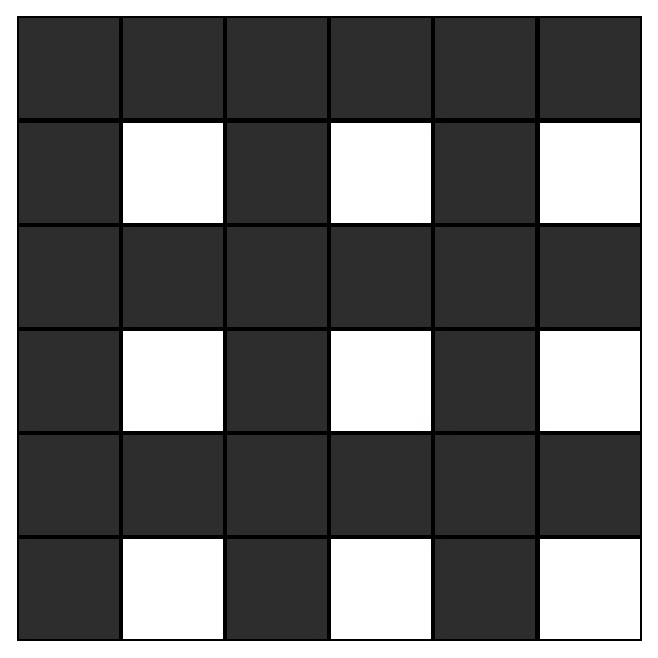
\includegraphics[width=3cm]{example_pattern}
%\caption{An example of a black and white pattern}
%\label{fig:example_pattern}
%\end{figure}

A rectangle strip-rule on $P$ is either a black or white rectangle that extends from one side of the pattern to the opposite side.
Precisely a rectangle in $P$ is either a set of contiguous rows of $P$ or a set of contiguous columns of $P$

A rectangle strip-rule list (a SRRL) that generates $P$ is an ordered list of rectangle strip-rules, that when applied in ordered to a blank (white) grid the size of $P$ create the target pattern. See Fig.~\ref{fig:pattern_generation} for an example of a pattern generated by a SRRL.

\begin{figure}[h]
\centering
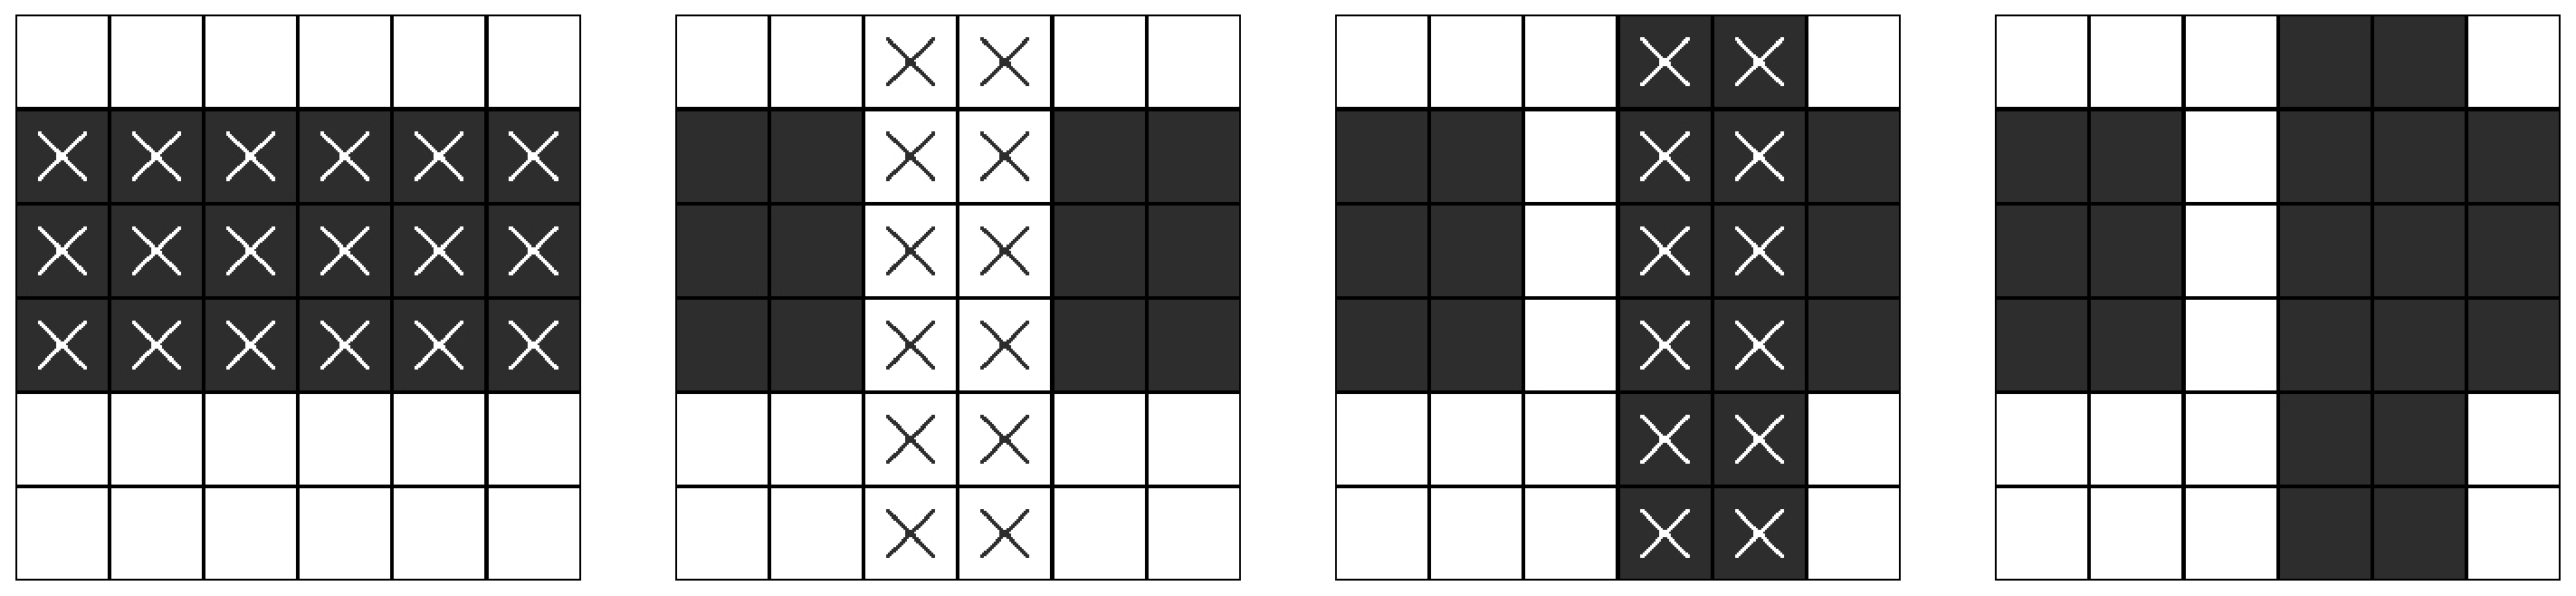
\includegraphics[height=3cm]{pattern_generation}
\caption{A pattern generated by a SRRL of 3 elements}
\label{fig:pattern_generation}
\end{figure}

We say a pattern $P$ is a strip-rule pattern if there is a SRRL that generates $P$. Note that not every pattern $P$ is a strip-rule pattern. See Fig.~\ref{fig:checkerboard} for an example of a pattern that is not a strip-rule pattern.

\begin{figure}[h]
\centering
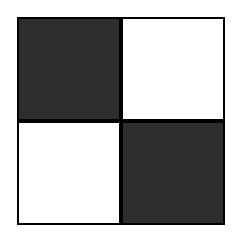
\includegraphics[width=1.5cm]{checkerboard}
\caption{The $2 \times 2$ checkerboard: an example of a pattern that is not a strip-rule pattern}
\label{fig:checkerboard}
\end{figure}

% Our goal on this paper is, given a pattern $P$ of dimensions $n_{R} \times n_{C}$, finding if $P$ is a strip-rule pattern and, if so, finding a minimal SRRL for it.

An SRRL is considered optimal if it has the minimum number of rectangle strip-rules of any SRRL that generates $P$.


\subsection{Problem Background}

\subsubsection{Rectilinear Pictures and Access Control Lists.}
The method of stacking rectangles to create patterns has applications in both graphics and network routers.
A common method for drawing graphics is to allow the user to repeatedly apply a rectangle tool to a blank canvas (See Xfig or PowerPoint).
Each rectangle is of a solid color and covers everything in a defined rectangular region.
This sequence of rectangles drawn can be represented by a rectangle rule list (RRL).
The problem of finding the minimum length RRL needed to create a given pattern is a generalization of the SRRL problem we explore.

Alternatively, instead of being given an $n_{R} $ by $n_{C}$ grid as input,
one can start with the numbers $n_{R}$ and $n_{C}$, and a list of $m$ rules.
The goal is to find a minimum-length list that gives the same pattern as the
input list. As shown in an extended version of \cite{ACJKLW07},
it is possible to
construct the $n_{R} $ by $n_{C}$ grid in time $O(n_R \cdot n_C + m^2)$.

One important application of RRLs is in access routers.
An Internet Service Provider might use access control lists (ACLs) on network router line cards in order to choose whether to forward or drop a packet based on the sending or receiving IP address.
This decision could be answered by checking a two-dimensional Boolean array based on the sender and receiver IP addresses.
This problem can be translated into a restricted version of our RRL problem.
An in depth discussion of this translation and its properties is discussed in detail in "Applegate et al."'s paper \cite{ACJKLW07}.
In ACLs minimization, the rectangles are of the certain form:
$n_R$ and $n_C$ are powers of two, rows and columns are
indexed with binary strings
from $0^w$ to $1^w$,  and each rectangle must be given by
two prefixes $y$ and $z$ of length at most $w$ each;
the actual rectangle consists of the rows whose index has
 $y$ as a prefix and the columns who have $z$ as prefix.



\subsubsection{Related Work.}
Unfortunately, the general problem of finding minimum length RRLs has been shown to be NP-Hard by \cite{ACJKLW07}.
Instead, we work on a restricted version of the problem in which any rectangle rules applied must extend either the height or width of the original pattern and only black or white rectangles are allowed.
This 2-color strip-rule problem was originally posed in "Applegate et al."'s paper
\cite{ACJKLW07}, where an optimal solution is given in $O(n^3)$-time, where $n$ is the sum of the height and width of the original pattern.
\cite{ACJKLW07} obtains an optimal solution to the strip-rule version of the
ACL problem with a similar (but more complicated) $O(w n^3)$-time algorithm.
A 1.5 ratio approximation algorithm is given for the problem in $O(n^2)$-time.
While there exist numerous results related to various other restricted problems regarding RRLs, we know of no other work related to this 2-color strip-rule problem.

ACL can be used in firewalls \cite{KRRW12}.
\cite{KRRW12b} introduce axioms with the goal of
creating and analyzing algorithms for optimizing the rewriting of rules
in Software Defined Networks.
\cite{LMT10} consider classifiers in dimensions higher than two,
which reduce to either ACL or RRL lists in dimension two. They propose
and experimentally evaluate heuristics without performance guarantees,
as well as relate these classifiers to the Firewall Decision Diagrams of
\cite{GL07}.
\cite{PL14}, and \cite{CDG16}  also consider higher dimensional classification based on rules.
\cite{KLRW13} and \cite{ZNHBM14} introduce more general rule-minimization problems.
\cite{SK10} uses rule minimization as a start for solution to an
extended problem. Efficiently
removing redundant rules has been proposed in \cite{SK10b}.

The complexity of finding minimum length ACLs in two dimensions
is still unknown, but with an arbitrary
number of dimensions, this problem is NP-hard \cite{KNCER13}.
\cite{ACJKLW07} gives a $O(\min(m^{1/3},\OPT^{1/2}))$-approximation
algorithm for finding minimum length RRLs, where $m$ is the length
of the input $RRL$. This is still the best published ratio.

\cite{DLT16} provides heuristics for higher-dimensional ACL and RRL
minimization
(\cite{DLT16} calls the ACLs minimization prefix-ACL, while
range-ACL is their terminology for finding minimum length RRLs),
on the way improving the approximation ratios provided by
 \cite{ACJKLW07} for ACLs minimization.  The approximation
algorithms of \cite{DLT16}  and \cite{ACJKLW07} use
as a subroutine the strip-rule version that we study.


\subsubsection{Our Results.}
Using the structure defined in "Applegate et al."'s \cite{ACJKLW07}
$O(n^3)$ exact algorithm for 2-color SRRLs,
we give an improved $O(n^2 $ log $n)$ exact algorithm for the SRRL problem.
Given the similar structures of the RRL and ACL optimal solutions given by
\cite{ACJKLW07}, we expect our solution can be extended to improve the
running time of an exact algorithm
for the strip-rule ACL problem from $O(wn^3)$ to  $O(w n^2$ log $n)$.
As strip-rule ACLs occur in high percentage
of ACL minimization cases \cite{ACJKLW07}, this is one reason to study SRRL.
Another two reasons are: we believe SRRL is a natural problem, and  SRRL is used in the approximation algorithms for RRL minimization.

Our result is obtained by digging deeper in the structure of the
dynamic programming of \cite{ACJKLW07} combined with use of
geometric data structures to speed up the process.
We use fast two-dimensional orthogonal range queries,
using existing data structures  (a time bound of $O(\log n)$ time
 per query being textbook material \cite{KOS2000}).



\subsection{Organization}
We begin by defining all structures and concepts relevant to finding the optimal SRRL.
Next we give a detailed explanation of our $O(n^2$ log $n)$ optimal algorithm.
Finally, we state all theorems that make the algorithm possible and analyze the algorithm's time and space complexity.

\section{Preliminaries}

We begin by exploring the strategies and tools for finding an optimal SRRL. The Pick-Up-Sticks algorithm will detail the basic structure used to find an SRRL, but not necessarily the optimal SRRL. Then we will explain the concept of equivalence classes, which can be grouped into segments. All of these concepts will be put together in our algorithm for finding the optimal solution.


\subsection{The Maximum Pick-Up-Sticks (MPUS) Algorithm}

As proposed by "Applegate et al."'s paper, we can build an algorithm for finding whether a pattern is a strip-rule pattern and, if so, finding an SRRL that generates it.

\subsubsection{The Pick-Up-Sticks (PUS) Algorithm.}

The Pick-Up-Sticks algorithm of \cite{ACJKLW07}
 is an algorithm for generating a SRRL of a pattern P if such a list exists. The idea is to pick up monochromatic rows and columns in order to build the SRRL backwards. Every time we pick a row or column, we color it gray.

Let $P$ be a black and white pattern. We define a column or row in P as being pseudo-monochromatic if it is composed of only gray and white cells or black and gray cells. Note that monochromatic columns and rows are also pseudo-monochromatic.

The Pick-Up-Sticks algorithm builds an SRRL as follows:

While there are still
black cells, choose a pseudo-monochromatic column or row and color all its cells gray. After a row or column is colored gray, add a rectangle that corresponds to covering that row or column with whatever non-gray color was left in that row or column to the beginning of our SRRL.
Note that, in our problem definition,
 we begin applying SRRLs with a white grid, so we can stop
picking up sticks when no black cells exist.
If, on the other hand, we modify the problem to begin with a grid of some
third color, we would only stop picking up sticks when all cells are gray.
There may be a difference of one rule between the optimum solutions to these two
problems (white grid or some third color grid) with the same target pattern.
For the sake of symmetry, from now on we use this {\em modified version}
of the problem. The method works with minor modifications for
the original version.

The algorithm may not succeed,
as it may not find a pseudo-monochromatic column or row.
If the algorithm does end in a all-gray grid,
%the algorithm has found a SRRL for the pattern $P$. If not, $P$ is not a strip-rule pattern. For the successful case,
the algorithm has "picked up" the rectangles of the SRRL in reverse order. Figure~\ref{fig:pick_up_sticks_example} gives a representation of one possible execution of the Pick-Up-Sticks algorithm and Fig.~\ref{fig:pick_up_sticks_srrl} shows the generation of the original pattern from the resultant SRRL.

\begin{figure}[h]
\centering
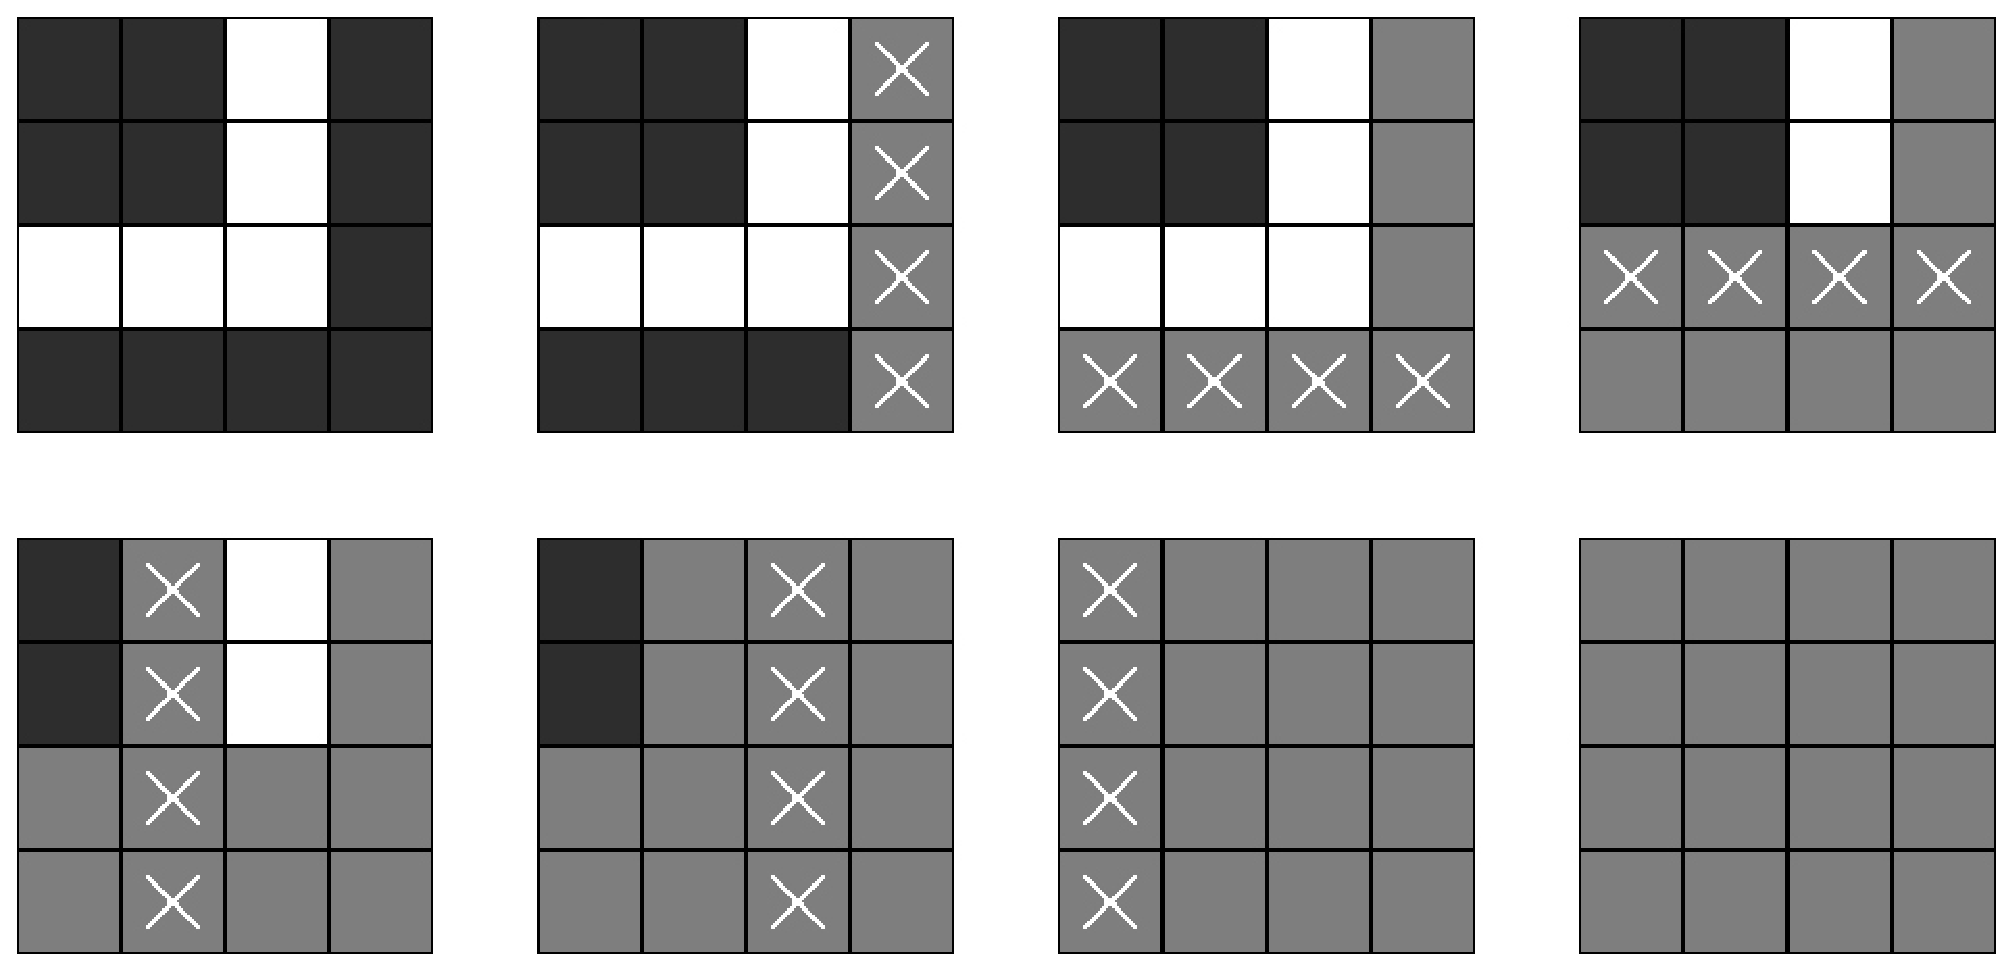
\includegraphics[width=10cm]{pick_up_sticks_example}
\caption{The execution of the Pick-Up-Sticks algorithm on a strip-rule pattern.}
\label{fig:pick_up_sticks_example}
\end{figure}

\begin{figure}[h]
\centering
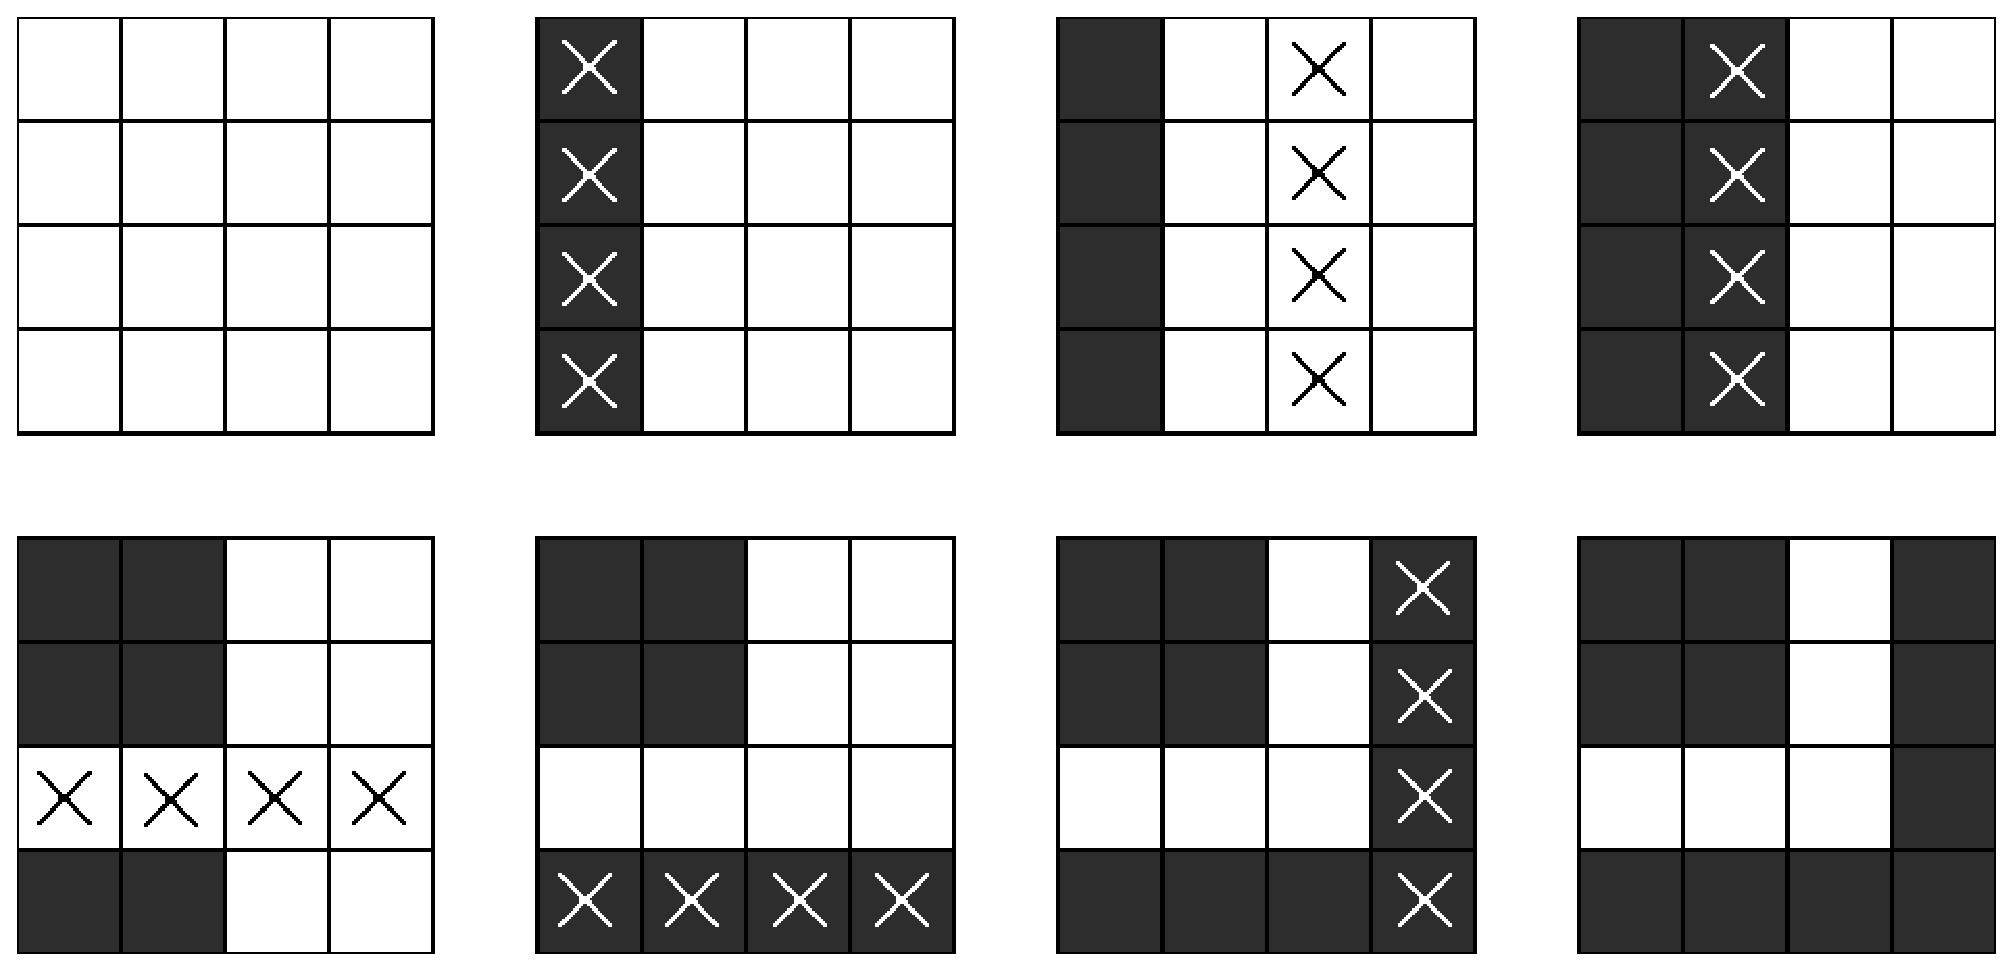
\includegraphics[width=10cm]{pick_up_sticks_srrl}
\caption{The SRRL generated by the execution of the MPUS algorithm on the pattern of the Figure~\ref{fig:pick_up_sticks_example}.}
\label{fig:pick_up_sticks_srrl}
\end{figure}

The Pick-Up-Sticks algorithm is guaranteed to generate an SRRL if one exists
\cite{ACJKLW07} (included in Appendix, Subsection \ref{corr_pus}), but it is not necessarily the optimal SRRL of minimum length. At any stage of the algorithm there will be more than one option on which row or column to pick up. Different choices can lead to different sizes of SRRLs. In the next sections we will discuss on how "Applegate et al."'s paper narrows down the number of choices for each stage in order to find the minimal SRRL.

\subsubsection{Improving by Picking Maximal Sticks.}

One important observation by "Applegate et al."'s paper on the Pick-Up-Sticks (PUS) algorithm is that there can be no harm in always using maximal strip-rules. A maximal strip-rule is a strip-rule that picks up a maximal contiguous sequences of pseudo-monochromatic rows or columns. Following \cite{ACJKLW07},
we call such a contiguous sequence a {\em block}.

This is possible because replacing a non-maximal strip-rule by the maximal one that contains it does not affect the pseudo-monochromaticity of any later rule.

Hence, we may always use the Maximal Pick-Up-Sticks (MPUS) algorithm instead of the Pick-Up-Sticks (PUS) algorithm. In this new algorithm, once we choose the pseudo-monochromatic column to pick, we pick the maximal contiguous set of pseudo-monochromatic columns that contains it.


\subsection{Equivalence Classes}
\label{ss_equiv}

We now introduce the concept of equivalence classes, as proposed by "Applegate et al."'s paper. This definition will allow us to give structure on the order of which columns and rows should be picked-up during an execution of MPUS in order to find an optimal SRRL.

\subsubsection{Definition and Properties.}
Given a pattern P, we define two rows or columns as being of the same equivalence class if and only if they are both of the same type (row or column) and their cells have the exact same colors in P, in the same order; that is, they are identical.

We will denote a column equivalence class in a pattern $P$ as being $C_{x}$ where $x$ is the number of black cells in the original pattern. Analogously, we will denote $R_{y}$ as being the row class with $y$ black cells in the original pattern. See Fig.~\ref{fig:equiv_classes_example} for an example of a pattern and its equivalence classes.
It follows from the monotocity property (Theorem
\ref{theorem_strip_rule_patterns}
in Subsection \ref{ss_monoton} of the Appendix)
 that all the columns in $C_x$ are identical in all
positions, for all $x$, and the same property holds for all the rows of $R_y$,
for all $y$.

\begin{figure}[h]
\centering
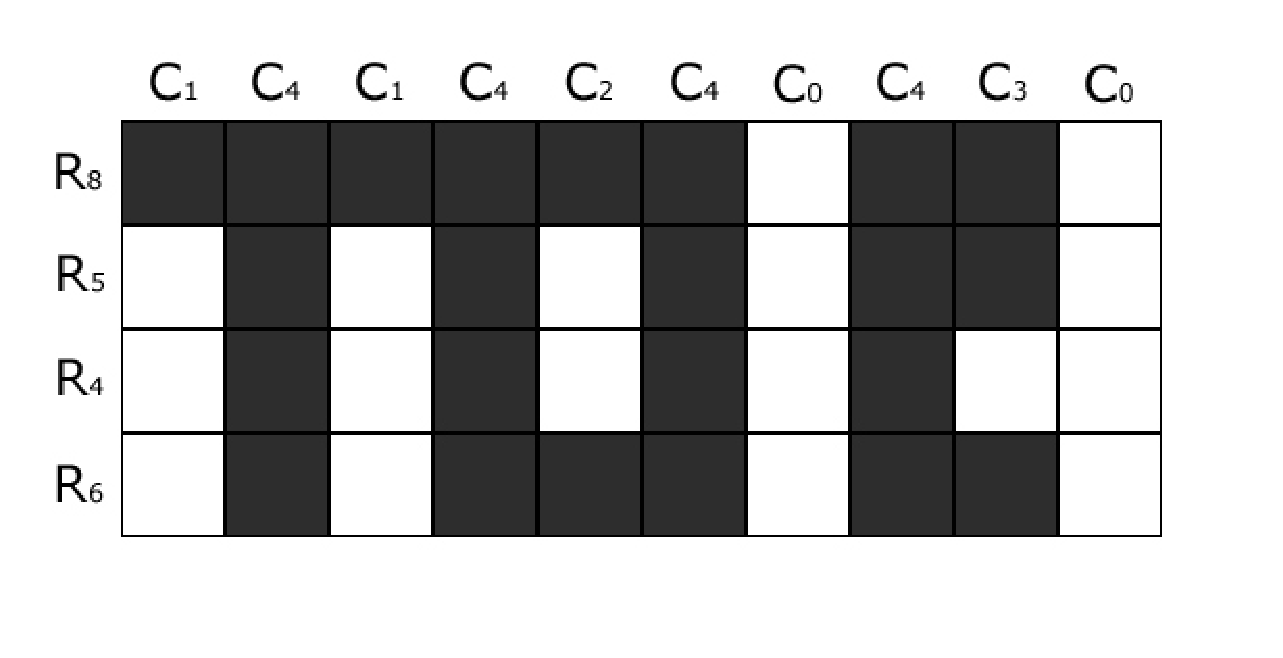
\includegraphics[height=5cm]{equiv_classes_example}
\caption{Equivalence classes of a black and white pattern P.}
\label{fig:equiv_classes_example}
\end{figure}

Note that every row and column belongs to exactly one equivalence class. Also, if two columns belong to a equivalence class in the beginning of the MPUS algorithm, they will remain of the same class until one of them is picked up
by the algorithm. This is since picking up other columns does not
change these two columns at all, while picking up rows modify these
two columns in exactly the same way. The same property holds for two
rows that belong to a equivalence class.

 %the very end of its execution. This will be proven later,
 %but the idea is that if any cell of row or column is removed,
 % the same cell will be removed for every member of its equivalence class.

We also define an equivalence class as being {\em active} during the execution of the MPUS algorithm if some member of that class is pseudo-monochromatic
but not all gray.

\subsubsection{Active Classes Properties.}
"Applegate et al."'s paper shows that during the execution of the MPUS algorithm on a black and white strip-rule pattern, there are always exactly two active classes at any given time.
The intuition on why this happens is that in order for a new class to become active, all the members of an old active class need to be picked up.
A formal proof of this property appears later in
Proposition \ref{t_active_classes} in the Appendix
(Subsection \ref{ss_classes});
this fact is also used in \cite{ACJKLW07}.
Also, the same proposition shows that
the two active classes are either a row and a column
class of the same color or both classes of the same kind (rows or columns),
 being one of each color.

\subsubsection{Embedded Rows and Columns.}
We can start improving the MPUS algorithm by introducing the concept described by "Applegate et al."'s paper as embedded rows and columns. This will allow us to pick up more rows and columns using the same number of rectangles.

First, we will define the concept of a embedded column or row at a given stage of the MPUS algorithm.
Given a point during the execution of the MPUS algorithm,
let $b$ be a column of an active equivalence class $B$.
Let $a_{1}$ be the first column to the left of $b$ that does not belong to $B$ and has not yet been picked up.
Similarly, let $a_{2}$ be the first column to the right of $b$ that does not belong to $B$ and has not yet been picked up.
We say that $b$ is {\em embedded}
 in equivalence class $A$ if both $a_{1}$ and $a_{2}$ belong to that class $A$. The definition is analogous for rows. Note that columns can be embedded only in column classes and rows only in row classes. See the three leftmost columns of Fig.~\ref{fig:embedment_example} for a simple example of a white column embedded in two black columns.

\begin{figure}[h]
\centering
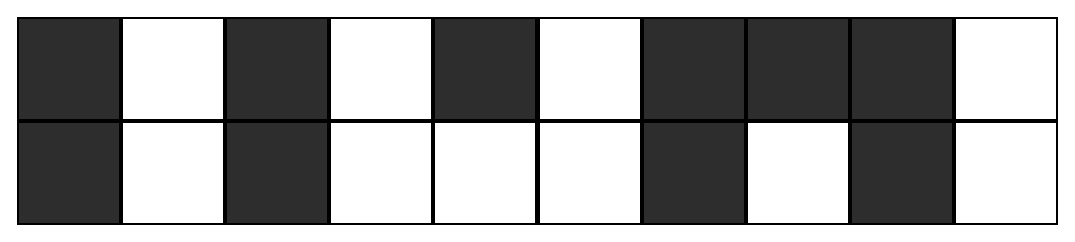
\includegraphics[width=10cm]{embedment_example}
\caption{Example of a pattern $P$ where some members of $C_{0}$ are embedded in some members of $C_{2}$.}
\label{fig:embedment_example}
\end{figure}

If during the execution of the MPUS algorithm we have the option to pick up two
column-blocks that embeds a set of columns of another class,
 we could pick up the two column-blocks that embeds the third one with
 two rectangles and then the embedded one, totaling three rectangles.
 However, it is better to pick the embedded block first with one rectangle,
and then pick the two blocks that were previously embedding with only one
rectangle, thus using a total of two rectangles for the same set of columns.
As an example, in Fig.~\ref{fig:embedment_example}, one cannot benefit
by picking up the first and the third column, when one can pick up
first the second column, followed by picking up the block of the first three
columns.

\subsubsection{Equivalence Classes Ordering.}
\label{ss_ordering}
As we pick up all the members of a column class, we change the rows of the pattern. Since the other columns remain intact, the new class to become active must be a row class. By using the same argument for row classes, we see that whenever we pick up all the members of a class, the next class to become active is of the opposite type.  This is formally proven in Proposition
\ref{theorem_pick_up_altertation} in the Appendix.
Also (same proposition), if we pick up all the members of an active class that was pseudo-monochromatic on a given color (for instance, black), the next class to become active needs to be of the opposite color (for instance, white). This happens because if it was of the same color, the other class would already have been active.

We can order the equivalence classes of both rows and columns in a given
 pattern $P$ by the number of black cells on it. In that ordering,
we can see (Proposition \ref{theorem_difference_is_class} in the Appendix)
that the all the rows that two consecutive column classes differ
 form exactly an equivalence class. This holds analogously for columns.
This implies (Proposition \ref{lemma_num_rows_col_differ_one} in the Appendix)
that the numbers of columns and rows classes differ
by at most one.  Using that information,
 we can set up the following ordering for the equivalence classes
(see also Proposition \ref{corollary_hierarchical_sequence} in the Appendix):

\begin{enumerate}

\item Start with the column class with only white cells. If such class does not exist, start with the row class with only black cells  (the existence of
this row class follows immediately from the monotonicity property -
Theorem \ref{theorem_strip_rule_patterns} in the Appendix).

\item Alternate columns and rows, putting the columns in ascending order of black cells and the rows in descending order of black cells.

\end{enumerate}

Let $C_{x_{0}}, C_{x_{1}}, \cdots, C_{x_{(N_{C}-1)}}, C_{x_{N_{C}}}$ be the ascending ordering of column classes by the number of black cells. Let $R_{y_{0}}, R_{y_{1}}, \cdots, R_{y_{(N_{R}-1)}}, R_{y_{N_{R}}}$ be the ascending ordering of row classes by the number of black cells. Using the rules above, we should get an ordering similar to $C_{x_{0}}, R_{y_{N_{R}}}, C_{x_{1}}, R_{y_{(N_{R}-1)}}, \cdots, R_{y_{1}}, C_{x_{(N_{C}-1)}}, R_{y_{0}}, C_{x_{N_{C}}}$. We will call this ordering the {\em hierarchical array} of the pattern $P$. We will also refer to this ordering of equivalence classes as $E_{1}, E_{2}, \cdots, E_{N}$.
Note that $N_C$, the number of column classes, is at most $n_C$,
the number of columns, and the same property holds for rows.

One important property of the hierarchical array of a pattern is that if $E_{x}$ and $E_{y}$, $x < y$, are the active classes during the MPUS execution, all classes that come before $E_{x}$ in the sequence or after $E_{y}$ must have already been picked up (otherwise, $E_{x}$ and $E_{y}$ would not be active).
This is proven in Proposition \ref{corollary_hierarchical_sequence}
in the Appendix.
Also from \ref{corollary_hierarchical_sequence}, if a class is between those two classes, none of the rows/columns of the in-between class
are pseudo-monochromatic.
The hierarchical array is a useful extension of Observation 5 on page
1070 of \cite{ACJKLW07}.


\subsection{Segments}

During MPUS, there are always two active classes. A ``segment"
succinctly represents the blocks that are available for pick up
while a certain pair of classes are active.
These segments can be translated into nodes of a graph, that can be used for finding the optimal solution, as described below. Note that our representation of segments is a slightly condensed version of the one described in the original
"Applegate et al."'s paper \cite{ACJKLW07}. The difference is that
the original definition is a five tuple with two redundant fields.
See Subsection \ref{ss_seg} of the appendix for a proof that these fields are
redundant. It is not here where the running time is improved.

\subsubsection{Definition and Properties.}

Whenever a new class becomes active during the execution of the MPUS algorithm
 on a pattern $P$, we will define a {\em segment} $S$ as being a tuple of
three elements $(E_{x},E_{y},U)$ where $E_{x}$ and $E_{y}$ are the active
equivalence classes and $U$ is the subset of members (rows or columns)
 left unpicked of $E_{y}$ ($U \subset E_{y}$).

We can represent the sequence of actions of the MPUS execution as
a sequence of segments, as described in this paragraph.
 Given the pick-up order obtained through the execution of the MPUS,
let's create a segment $(E_{0}, E_{N}, E_{N})$ for the starting state of pattern $P$ and a segment $(E_{x}, E_{y}, U)$, $U \subset E_{y}$, for every time a new class $E_{x}$ becomes active; we say that the SRRL {\em includes} the
segment whenever such a segment becomes active during the MPUS execution
corresponding to the SRRL.

Since $E_{x}$ is the new class, all of the members of $E_{x}$ are still in the pattern. $E_{y}$, in the other hand, is a class that was already active. It may have some of its members already picked-up. We store that information in $U$ by maintaining the members that have not been picked up yet. Note also that any classes that are between $E_{x}$ and $E_{y}$ in the hierarchical array of $P$ have not become active yet, resulting in the fact that all of
their members are still there. At the same time, members that come before and after the interval delimited by $E_{x}$ and $E_{y}$ have all been picked up. Hence, for each one of those segments that are created whenever a class becomes active it is possible to reconstruct the pattern at that moment of the execution of the MPUS algorithm.

\subsubsection{Segment Branching.}

"Applegate et al."'s paper \cite{ACJKLW07}
shows that if we are looking for an optimal solution we can narrow down the number of segments significantly by reducing the number of options a segment can branch to two.

Suppose a minimum-length SRRL for a strip-rule pattern $P$ includes the segment $S = (E_{x}, E_{y}, U)$ and that to get to the next segment, if it exists, we pick up all members of $E_{x}$
(possibly picking up some members of $U \subset E_{y}$)
while at least one member of $U$ remains active.

\begin{itemize}

\item If $U \subset E_{y}$ has a member that is not embedded in $E_{x}$,
 there exists a minimum-length SRRL that includes the segment
$S = (E_{x}, E_{y}, U)$ and that to get to the next segment you pick up
 all the members of $U \subset E_{y}$ that are embedded in $E_{x}$,
 followed by picking all members of $E_{x}$.

\item If all members of $U \subset E_{y}$ are embedded in $E_{x}$,
 there exists another minimum-length SRRL that includes the segment
$S = (E_{x}, E_{y}, U)$ and that to get to the next segment you
 pick up all the members of $U \subset E_{y}$
(thus, finishing picking up every member of $E_{y}$ in the pattern).
Note that in this case, one can get to the next segment by picking up all
the members of $U \subseteq E_y$ first.

\end{itemize}

The same property holds with the roles of $E_{x}$ and $U$ switched. In this case, we assume the next segment from $S$, if it exists is originally reached by picking up all members of $U \subset E_{y}$.

This happens because we can always pick embedded members at no extra cost,
if one is to pick all the blocks of the embedding class, as shown in
Proposition \ref{p_embed} of the Appendix.
Moreover, suppose we have two sets $U_x$ and $U_y$
of active blocks of the two active classes $E_x$ and $E_y$.
To finish picking up blocks (except at the very end), we must
reach the situation that either $E_x$ or $E_y$ are not active anymore;
say $E_x$ becomes not active, while $E_y$ is still active.
%together with a new active class $E_z$.
Picking up any block from the class $E_y$ that is not embedded in $E_x$
can be done, without loss of optimality, later.
So we can assume that
 only the members of $U_y$ that are embedded in $E_x$ are picked up
while $E_x$ is active.

 Note also that for every segment we could pick the latest class that became active or the oldest, a total of two options. We can then say that every segment will branch into two other segments. On both cases, we can determine the next segment reached by eliminating every embedded member of the class not being picked-up, followed by eliminating every member of the class being picked-up. The only exception to this, is if when we pick every embedded member of the class not being picked-up we end up picking all of its members, thus already reaching a new segment. In that case, the original segment branches into only one segment, instead of two.

Note that there could be a segment that does not have any next segment. In this case, the segment is a segment at the very end of minimum-length SRRL. If we pick up any of either class, we will obtain an all-gray grid and the algorithm will be over. Also, note that for this to happen we must have that $E_{x}$ and $E_{y}$ are next to each other in the hierarchy array, and picking-up one of them will also result in picking-up the other one.

\subsubsection{Segment Graph.}

We build a graph using the segments as nodes, as described by the following structure proposed by \cite{ACJKLW07}:

\begin{itemize}

\item Start with the segment $(E_{0}, E_{N}, E_{N})$, that represents the grid as it is in very beginning of the MPUS algorithm. This will be the starting node.

\item For every node (segment) in the graph, generate the two segments (possibly one, as described in the previous subsection) that it branches into and add a directed edge from it to the new generated nodes.
 There will be one segment for each of the two options of picking up the newest or the oldest of the two classes in the segment. On both cases, we can determine the next segment reached by eliminating every embedded member of the class not being picked-up, followed by eliminating every member of the class being picked-up.

\item Define the cost for each edge as the number of rules in the MPUS algorithm used to go from one segment to another.

\item Create an artificial node corresponds to an all-gray grid. This will be the end node of the graph. Every time a segment has its two classes adjacent to each other in the hierarchy array, create an edge from it to this all-gray grid node.
 This edge should have cost one (since we solve the modified version);
if we were to solve the original version, this edge should have cost zero
if the members of the classes of the segment were white and one otherwise.

\end{itemize}

Because of what was discussed in the Segments Branching section, at least one of the paths from the starting node to the end node of the graph will be a minimum-length SRRL.
 Note that having $(E_{N}, E_{0}, E_{0})$ as the starting node will lead to a graph that represents the same possible steps for the MPUS because it also represents the same starting pattern. Note also that some nodes may be reached by more than one node. Every node will only branch into nodes that correspond to patterns with fewer total of columns and rows. This implies that there are no cycles in this graph.

We say that one segment reaches another if there is a path in this graph from that segment to the other one. The distance from one segment to another is the sum of the costs of the edges that compose the path between them, if such exists.

One very important property of this graph that will be proven later is that if two segments $(E_{x}, E_{y}, U)$ and $(E_{x}, E_{y}, U')$ are reachable from the the starting node of the graph, then either $U \subset U'$ or $U' \subset U$. This property will be referred as the Containment Lemma and appears
in Subsection \ref{ss_cont} in the Appendix. We will see that this implies that the number of nodes in this graph is $O(n^{2})$ where $n$ is the number of rows and columns in the original pattern.





\newcommand{\hs}{\hat{s}}
\newcommand{\hS}{\hat{S}}
\newcommand{\hU}{\hat{U}}

\section{Algorithm}
The flow of our algorithm closely follows that of the $O(n^3)$ algorithm given by "Applegate et al.".
We similarly create a segment graph of the reachable states in a MPUS of the pattern.
However, we create this graph faster by grouping similar segments into S-groups, which can be processed together.

\subsection{Setup}
We begin by reading the input pattern into an equivalence class list and creating the first node in our segment graph.

\subsubsection{Equivalence Class List.}
 We are given as input an $n_R \times n_C$ grid of black and white cells.
Assign each of the rows an index from 1 to $n_R$ from top to bottom, similarly each column, an index from 1 to $n_C$ from left to right.
 Group rows and columns into equivalence classes and order the classes by number of black cells as previously described in the Subsection \ref{ss_equiv}.
Precisely, construct the hierarchical array:
$$C_{x_{0}}, R_{y_{N_{R}}}, C_{x_{1}}, R_{y_{(N_{R}-1)}}, \cdots, R_{y_{1}}, C_{x_{(N_{C}-1)}}, R_{y_{0}}, C_{x_{N_{C}}}$$
(this array may start and/or end with row equivalence classes, instead of columns as above).

We will need to determine from a range of column indexes which columns are
also in a range of equivalence classes, and the similar question with
rows instead of columns.
A data structure such as an orthogonal range tree \cite{KOS2000}
accomplishes these queries in $O($log $n)$ time with $O(n \log n)$
space and setup time.

\subsubsection{S-group.}
 %All of this is definition of segment and doesn't need to be here.
% We know that an optimal solution exists in the form of an MPUS.
% Any RRL created by MPUS can be divided into a sequence of segments, each segment containing all the rules applied when a given pair of equivalence classes were active.
% A segment can be uniquely identified by the 3-tuple label $\{E_1,E_2,U'\}$, where $E_1$ and $E_2$ are the active classes at the time of the segment, and $U$ is the set of members of $E_2$ which have not yet been picked up.
% (No members of $E_1$ will have been picked up because it has just become available for pick-up.) %Note this language has been heavily lifted from "Applegate et al.".
 Define an S-group $(E_1, E_2)$
(for equivalence classes $E_1$ and $E_2$, where the order of $E_1$ and $E_2$
in the tuple above matters)
 to be a collection of all segments $\{C_1,C_2,U'\}$
such that $C_1 = E_1$ and $C_2 = E_2$.
 To completely represent each of these segments, an S-group $(E_1, E_2)$
maintains a list of segments $S$ and a master list $U$.
 This list $U$ will be used to keep track of each of the segment's individual
 list $u$, as described below.
 This allows each segment to be stored in constant space, while the S-group gets stored in $O(|E_1|+|E_2|)$ space.

 The list $U$ contains the index of every member of $E_2$ ordered such that for every segment $\{E_1,E_2,U'\}$ in the S-group, the first $|U'|$ members of $U$ comprise the same set as $U'$.
Such an ordering is guaranteed to exist by the Containment Lemma from
 Subsection \ref{ss_cont}.
We generate this ordering by noting that indexes appearing in more segments appear earlier in the list $U$.

$S$, the list of segments maintained by the S-group, keeps these
segments ordered by the size of their set $U'$.
Each segment $s_i$ will have three values, $u(s_i)$, $d(s_i)$, and $p(s_i)$.
$u = |U'|$.
%We can ignore any segment with $u=0$ by OPTIMAL SEGMENT LEMMA, so we will assume $u>0$.
$d$ gives the minimum number of sticks required to reach the state of segment starting from the original pattern.
We want to maintain the shortest path to each node, so we use the value $p$ to store a reference to the segment right before this one on this path. %WOrding. I dont know how to say this better.

%Finally we create an $n \times n$ array to store our S-groups.
\subsubsection{Origin S-group.}
We begin with the S-group $(E_1,E_2)$ with $U = \overline{E_2}$ and $S$ comprised of a single segment $(u,d,p) = (|\overline{E_2}|,0,null)$, where  $\overline{E_2}$ represents the complete set of the members of $E_2$.
The classes $E_1$ and $E_2$ are the first and last members of the
hierarchical array.
We will explore outwards from this S-group in a breadth first fashion, enumerating all reachable segments.
The graph on the S-groups is guaranteed to be acyclic because the number of picked up classes is strictly increasing along each edge.




\subsection{Finding the Next S-group}


Suppose we have some S-group $(E_1, E_2)$ with associated lists $U$ and $S$.
Without loss of generality we will assume $E_1$ to be a column class.
We wish to generate all S-groups reachable from this S-group.
The two S-groups immediately reachable from this S-group correspond to completely removing either class $E_1$ or $E_2$.

To determine the cost of removing a class $E_i$ from a segment $s_j$,
we count how many members of $E_{3-i}$
can be picked up for free, as described in detail later.
If two members of $E_i$ may be picked up with the same stick
while $E_1$ and $E_2$ are the active classes, we will call the
two members {\em contiguous}. It follows from Proposition
\ref{corollary_hierarchical_sequence}
%and the discussion at the end of Subsection \ref{ss_ordering}
that a pair of columns is contiguous in an S-group $(E_1,E_2)$ if every column
between them is either already picked up or of type $E_1$ or $E_2$.

Before the class $E_i$ can be removed from a segment  $(E_1,E_2,U')$
(all the members of the class being picked up),
we pick up every embedded member of $E_{3-i}$.
To determine the cost of moving to the next segment,
we must count how many of the embedded columns are also contiguous.
Then any embedded columns must be removed from either
the set $U'$ (if $E_1$ is removed) or $E_1$ (if $U'$ is removed) in the next
segment and, by doing this for all segments, in the next S-group.
In fact, we process one S-group at a time, and obtain segments of
another at most two S-groups, as explained below.

Because $E_1$ and $E_2$ are not symmetric ($E_2$ comes with its set $U$), we will describe the process of removing classes $E_1$ and $E_2$ separately.

%Possibly move some more things here out of the E1 and E2 subsections

\subsubsection{Remove $E_1$.}
Let $E_3$ be the equivalence class adjacent to $E_1$ in the equivalence class list, which has not yet been removed.
The S-group corresponding to the result of removing $E_1$ will be $(E_3,E_2)$
with lists $\hU$ and $\hS$.

\paragraph{Count Contiguous Consecutive Pairs of Columns of $E_1$.}
To determine the distances to the segments of the next S-group,
we must count the number of contiguous $E_1$ ranges.

To do so, we must determine the range of equivalence classes which have not yet been picked up.
Let $E_1$ be the column class $C_a$.
If $E_2$ is also a column class call it $C_b$.
If $E_2$ is a row class, then $C_b$ is the column class adjacent to $E_2$ in the equivalence class list that has already been picked up.
%Note that this assumes padding the list with imaginary classes C_0 and C_m+1
We assume $a<b$, with the other case being symmetric.
By Proposition \ref{corollary_hierarchical_sequence},
 a column class $C_i$ has not been picked up if and only if $i\in (a,b)$.
%Notation here. a could be bigger than b, but this seems pretty clear to me.


For each pair of adjacent members of $E_1$ we check to see if
they are contiguous.
Precisely, for each member $e_i \in E_1$, we query our column range tree for members in the range $[a+1,b-1]$ with index in the range $[e_i,e_{i+1}]$,
where $e_{i+1}$ is the column of $E_i$ that has the smallest index
among those with index higher than $e_i$ ($e_{i+1}$ is the next column of $E_i$
after $e_i$).
Let $c$ be the number of pairs of consecutive members of $E_1$ which are also contiguous.
The value $(|E_1| - c)$ corresponds to the number of sticks required to completely remove $E_1$ after any embedded columns of $E_2$ are picked up.

\paragraph{Get Embedded $E_2$ Blocks.}
If $E_2$ is also a column class, we must count and remove any members of $E_2$ embedded in members of $E_1$.
Similar to the way we checked that columns of $E_1$ were contiguous, we will check if adjacent columns of $E_1$ are both contiguous and contain columns of $E_2$.
In order to accurately keep track of the cost to remove these embedded columns we must give each embedded column a tag based on which two columns surrounded the embedded column.
Two members of $E_2$ can be picked up with the same stick if and only if they have the same tag.

When an embedded column is found, tag it with the index of the $E_1$ column to its left.
Then add this column to a list, $B$, sorted by the column's index.
After we have found all of the embedded columns, we are ready to generate $\hU$ and $\hS$.

\paragraph{Build the Next S-group.}
Begin with $\hU$ as an empty list.
We also need a set $T$ to keep track of which tags have been accounted for.
Iterate through $U$, searching for each member $m$ of $U$
 in the set of embedded columns, $B$.
If $m\not \in B$, append $m$ to the end of $\hU$.
Otherwise add $m$'s tag value to the set $T$ if it is not already there. %Stronger way to say this?
Once we have checked all of the members $U'$  in a segment $s_i$
($U'$ being the first $u(s_i)$ elements of $U$) ,
add a new segment $\hs_i$ to $\hS$ with the following values.
$$u(\hs_i) = |\hU|$$
$$d(\hs_i)  = d(s_i) + |T| + |E_1| - c$$
$$p(\hs_i)  = s_i$$
(note that $|\hU|$ and $|T|$ are computed for the sets  $\hU$ and $T$ exactly
when finish processing the last element of $U'$ while iterating through $U$;
$\hU$ and $T$ can change later on).
If $\hS$ already contains a segment $\hs_j$ with $u(\hs_j) = u(\hs_i)$,
then keep only the segment with shorter distance $d$ in the set $\hS$,
 and remove the other one. %wording?
As an aside, one can see that if we don't remove duplicates,
if two segments from the same S-group $s_i$ and $s_j$ have
$u(s_i) > u(s_j)$,  then
$u(\hs_i) > u(\hs_j)$,  which is used in the proof of the
Containment Lemma (Subsection \ref{ss_cont} in the Appendix).

\subsubsection{Remove $E_2$.}
Let $E_3$ be the equivalence class adjacent to $E_2$ in the equivalence class list, which has not yet been removed.
The S-group corresponding to the result of removing $E_2$ will be $(E_3,E_1)$ with lists $\hU$ (whose elements are members of the class $E_1$) and $\hS$.


\paragraph{Count Contiguous Consecutive Pairs of Columns of $E_2$.}
To count contiguous ranges of $E_2$, we must count the contiguous ranges within each segment separately.  We use a counter $c$, initially set to $0$.
Fortunately, if a pair of columns is contiguous in one segment, it is also contiguous in all larger (with bigger value of $u$) segments.
For each index $u_j \in U$ (elements of $E$ are indices of columns),
 insert $u_j$ into a sorted list of indexes, $I$.
Get the predecessor and successor of $u_j$ in $I$ and check if these ranges from $u_j$ to its neighbors are contiguous.
If either of these ranges exist and are contiguous
 then this column can be picked up for free.
If not, we increment our cost counter $c$.
Once we have iterated over the first $u(s_i)$ blocks, we save the state of our counter in a value $c_i = c$.
This value corresponds to the cost to completely pick up the columns in the segment $s_i$ after any embedded members of $E_1$ have been picked up.
Proceed (with $c$ possibly increasing) until we finish the list $U$.


\paragraph{Get Embedded $E_1$ Blocks.}
If $E_2$ is also a column class, we must count and remove the embedded columns of $E_1$.
Each segment could have a unique number of embedded columns, where the larger the segment, the more columns can be embedded and the smaller the resulting segment will be in the next S-group.
As an aside, this is an argument used in the proof of the Containment Lemma
from \ref{ss_cont}.
To generate the ordering of $\hU$ and the values in $\hS$ and
we must carefully count the embedded columns.

We iterate through the columns of $U$ keeping track of which columns
 are embedded and will get picked up.
To help us with this task, we start with a sorted list $V$
of the indexes of $E_1$, an empty list for $\hU$,
 and a counter $d$, initialized to $d=0$,
 to measure the number of required sticks.
Also start with $B$, a set of columns of $E_1$, initialized as the empty set.

Similar to the way we counted contiguous blocks, for each column $u_i \in U$ we insert $u_i$ into a sorted list of indexes $I$.
Get the predecessor and successor of $u_i$ in $I$, called $u_j$ and $u_k$
respectively, if they exist (in which case $j < i$ and $k < i$).
%To avoid reading embedded columns more than once, we give each $u_i$ a right mark or a left mark if embedded columns to its right or left respectively have been picked up and accounted for.
%If the successor does not have a right mark, then we check if the range is contiguous.
%If so, we query for the list of columns embedded between $u_i$ and its successor.
%Do the same for the predecessor, checking for a left mark.
Use range search to check if $u_j$ and $u_i$ are contiguous,
and if $u_i$ and $u_k$ are contiguous; if a pair does not exist,
treat it as not being contiguous.
If neither of these two pairs is contiguous, do nothing.
If exactly one of these pairs is contiguous, use binary search in $V$
to obtain the set of columns of $E_1$ embedded between the pair,
add this set to $B$, and increment $d$.
If both of these pairs are contiguous, use binary search to determine
if there are elements of $\overline{E_1}$
(defined earlier as all the columns of class $E_1$)
 between $u_j$ and $u_i$ and between
$u_i$ and $u_k$; in which case we increment $d$.
%If any embedded columns were found increment $d$ and add the set of newly found embedded columns to set $B$ (which was initialized as the empty set).
After we have iterated through $u(s_i)$ columns of $U$, it is time to add to
$\hU$ and create a new segment $\hs_i \in \hS$ with the following values.
$$u(\hs_i) = |V| - |B|$$
$$d(\hs_i) = d(s_i) + d + c_i$$
$$p(\hs_i) = s_i$$ %Is it possible to end up with two segments of the same distance again? I dont want to think about it right now. @@
Remove all of the members of $B$ from $V$,
 then add all of these members to the beginning of $\hU$.
Reset $B$ to be the empty set.
Continue iterating through $U$.

Once we have finished iterating through $U$, add the remaining elements in $V$ to the start of $\hU$.

\paragraph{Build the Next S-group.}
If $E_2$ is a row class, then $\hU = \overline{E_1}$
 and $\hS$ contains one segment $\hs$.
To find $\hs$, we iterate over each segment $s_i \in S$
looking for the segment $s_i$ with minimum value $d(s_i) + c_i$.
$\hs$ has the following values:
$$u(\hs) = |\overline{E_1}|$$
$$d(\hs) = d(s_i) + c_i$$ %c_i doesnt make any sense here. c needs to be incorporated into the segments. ://///
$$p(\hs) = s_i$$ %you know, i still dont like the way i'm doing this. but I dont really mind breaking up the text. so i dont know.
%Maybe we incorporate the c_i thing into the segment similar to the rest.

If $E_2$ is a column class, $\hU$ and $\hS$
 were created while we found embedded columns.
%I could rewrite this so get embedded blocks actually returns the sets of embedded classes and then use it to compute next S-group in order to match the structure. This way seems easier if possibly harder or trickier.



\subsection{Merging Identical S-groups}

Once we have generated a new S-group $(E_1,E_2)$ we add it to a two dimensional table, where the row is determined by $E_1$'s index in the original list of equivalence classes, and the column similarly determined from $E_2$'s index.

If an S-group $(E_1,E_2)$ already exists, we must merge the two S-groups.
%At most three merges will occur for any given S-group type. Is this necessary here? This is more about the runtime.
Given two $(E_1, E_2)$ S-groups, $G_1 = \{U_1,S_1\}$ and $G_2 = \{U_2,S_2\}$, we will compute a new S-group, $G_3 = \{U_3,S_3\}$, that encompasses both of these S-groups which will then get stored in our table.
We iterate through both $G_1$ and $G_2$ concurrently in order to create $G_3$,
as described below. One starts with $U_3$ and $S_3$ being empty.


Merge $S_1$ and $S_2$, maintaining the ordering based on $u$
Iterate through each $s_i$ in this merged list.
Let $S_j$ be the list which contains $s_i$.
Remove elements from the start of $U_j$,
adding them to the end of $U_3$ until $|U_3| = u(s_i)$.
(Do not add a value to $U_3$ if it is already in $U_3$.)
This works because of the Containment Lemma from the
 Appendix \ref{ss_cont}. Actually, the proof in \cite{ACJKLW07}
of the Containment Lemma relies on proving the fact that
 all the values of $u(s)$ with $s \in S_1$ are at most the minimum
of the values of $u(s)$ with $s \in S_2$, or vice versa.
Add $s_i$ to $S_3$.
If $G_1$ and $G_2$ both have segments such that $u(s_a) = u(s_b)$, choose the segment of smaller distance to add to $S_3$.

\subsection{Finding the optimum SRRL}

While we build the graph, we keep track of the segment which is a valid endpoint of the smallest distance.
We define a valid endpoint to be a segment which is completely gray
(this is since we solve the modified version of the problem;
for the original problem, we would have a segment which is completely
white and gray).
A segment $(E_1,E_2)$, is an endpoint if $E_1=E_2$.
(in the original version, we also have the case where
$E_1$ and $E_2$ are adjacent in the equivalence class list and
 the cell where $E_1$ and $E_2$ intersect is white in the original pattern).
Then once the graph is finished, we build a path to the valid endpoint using the values stored in $p$.
This path will give the optimal order to remove equivalence classes, which can then be translated into the optimal list of rectangle rules.

This algorithms returns the optimum solution, as follows from all the
discussion above.

\section{Time and Space Complexity}
\label{s_run}


In this section we will show the time and space complexity of the previously defined algorithm is $O(nN$ log $n)$ and $O(nN)$ respectively -- where $N$ is the number of equivalence classes and $n$ is the number of rows and columns in the original pattern.
The ideas of our proof are partially taken from
a more complete version of \cite{ACJKLW07},
 which showed the number of reachable segments to be in $O(n^2)$.
Indeed, our contribution is a faster way of processing a segment,
cutting down this processing time down from $O(n)$ to $O(\log n)$.

Following \cite{ACJKLW07},
we will show that if the complexity for an S-group $(E_a,E_b)$ is in $O(|E_a| + |E_b|)$, then the overall complexity of all S-groups is $O(nN)$.
For each S-group, add the first term of its complexity, $O(|E_a|)$, to one two dimensional array, and its second, $O(|E_b|)$, to a second array -- each at location $(E_a,E_b)$.

\[
\begin{bmatrix}
    E_1 &  E_1 & \dots & E_1\\
    E_2 &  E_2 & \dots & E_2\\
    \vdots & \vdots & \ddots & \vdots \\
    E_N &  E_N & \dots & E_N\\
\end{bmatrix}
\begin{bmatrix}
    E_1 &  E_2 & \dots & E_N\\
    E_1 &  E_2 & \dots & E_N\\
    \vdots & \vdots & \ddots & \vdots \\
    E_1 &  E_2 & \dots & E_N\\
\end{bmatrix}
\]

By noting that the sum of all members of all equivalence classes equals the total number of rows and columns, we get $\sum_{i=0}^N{|E_i|} = n$.
The sum of the columns in the first matrix and the sum of the rows in the second matrix both equal $n$.
The sum of all terms in both matrices is $2nN$, so the complexity of all S-groups is in $O(nN)$.

The space complexity of the algorithm is determined by the sizes of the lists storing the S-groups.
Each S-group maintains a list $U$, which holds members of $E_b$,
 and is therefore in $O(|E_b|)$. The list $S$ contains all segments.
Each segment is guaranteed to have a unique size $u$,
and the values of $u$ are positive values less than $|E_b|$.
The complexity of each segment is constant, so we again have $O(|E_b|)$.
As we have previously shown, since each segment is in
$O(|E_a| + |E_b|)$, the overall complexity is $O(nN)$.

Each operation we perform on an S-group $(E_a,E_b)$ happens in time either
$O(|E_a|$ log $n)$ or $O(|E_b|$ log $n)$, as indeed
every ``check" from the algorithm's description takes time $O(\log n)$,
after $O(n \log n$ initialization of the range search data structure
or the ordered list represented by a balanced binary tree.
So the runtime for processing the equivalence class list is $O(nN$ log $n)$.

Since reading the input takes $O(n^2)$ time and $N$ is in $O(n)$
(this follows immediately from the Monotonicity Property,
 Theorem \ref{theorem_strip_rule_patterns} in the Appendix),
 we relax our bounds and say our space complexity is $O(n^2)$
 and the overall runtime is $O(n^2$ log $n)$.

\section{Conclusions}
\label{s_conc}
As noted in \cite{NLT13,NLT18}, these solutions do not generalize to
dimensions higher than two. This is the most interesting open question,
in our opinion.

%"We" means Gruia
We believe that range trees can be replaced by ad-hoc methods to
obtain a $O(n^2)$ algorithm for exact RRL strip-rule minimization.
The savings of $O(\log n)$ in running time comes at the expense
of a more complicated algorithm which we decided not to present.

\section*{Acknowledgements}
Ian's research done while at Illinois Institute of Technology, and supported by the Brazil Scientific Mobility Program.  
Gruia's and Nathan's work done while at Illinois Institute of Technology,
and supported by the National Science Foundation under awards NSF-1461260 (REU).



\printbibliography
\pagebreak

\section{Appendix}

%pick-up sticks correctness

\subsection{Correctness of Pick-Up-Sticks Algorithm}
\label{corr_pus}

For the sake of completeness, we include:
\begin{theorem} [part of Theorem 3.1 of \cite{ACJKLW07}]
\label{theorem_pick_up_sticks}
A black and white pattern $P$ is a strip-rule pattern if and only if the Pick-Up-Sticks algorithm results in a grid with  all of its cells gray. 
In that case, the reverse list of picked-up rows 
and columns is a SRRL for $P$.
\end{theorem}

Since Theorem 3.1 of \cite{ACJKLW07} is not proven in their conference version,
we include a proof for the sake of completeness.

\begin{proof}
Let's separate the proof into the two following parts:
\begin{itemize}
\item ($P$ is a strip-rule pattern) $\rightarrow$ (The Pick-Up-Sticks algorithm results in an all-gray grid)

Suppose $P$ is a pattern that can be generated by a SRRL 
$S = (s_{1},s_{2},\cdots,s_{m})$ of size $m$.  Suppose we have picked up some
sticks.
Let $s_{i}$ is the highest-index rule from $S$ that still has a 
row/column $c$ such that $c$ is not all-gray. 
If there is no such $s_{i}$, then we must have picked up everything. 
For every integer $j$, $i < j \leq m$, 
all the rows/columns of $s_{j}$ must have already been entirely colored gray.
That means that all cells of $c$ that belong to a rule $s_{j}$, with 
$i < j \leq m$, are gray. The cells of $c$ that are not gray must have
the same color as the rule $s_{i}$, as they will not be overwritten
by any rule $s_{j}$ with $i < j \leq m$. 
Hence, $c$ must be pseudo-monochromatic and then the Pick-Up-Sticks may proceed. As a result, the algorithm never gets stuck until the all-gray grid is reached.

\item (The Pick-Up-Sticks algorithm results in an all-gray grid) $\rightarrow$ ($P$ is a strip-rule pattern) 

The reverse list of the picked-up rows and columns is a SRRL since on every iteration of the algorithm we only pick up strips of $P$. If the Pick-Up-Sticks algorithm results in an all-gray grid, every row and column of $P$ has been picked up by the end of the algorithm. Hence, the reversed list of picked up rows and columns is a SRRL that generates $P$, making $P$ a strip-rule pattern.
\end{itemize}

This ends our proof.
\qed 
\end{proof}

The same proof works (the number of rules may differ by one) if
the Pick-Up-Sticks algorithm results in a grid with none of its cells black.


%monotonicity lemma comming next; maybe replace by citation


\subsection{The Monotonicity Property}
\label{ss_monoton}

\begin{theorem} [part of Theorem 3.1 of \cite{ACJKLW07}]
\label{theorem_strip_rule_patterns}
(Monotonicity Property) Let $P$ be a black and white pattern. $P$ is a strip-rule pattern if and only if the two equivalent properties holds:

\begin{enumerate}[(i)]
\item For any color $c \in \{black, white\}$, the rows of $P$ are hierarchical: given any two rows of $P$, the set of columns where $c$ is present in the first row either contains or is contained in the set of columns where $c$ is present in the second.

\item The same property of item (i) holds with the roles of row and column switched.
\end{enumerate}

\begin{figure}[h]
\centering
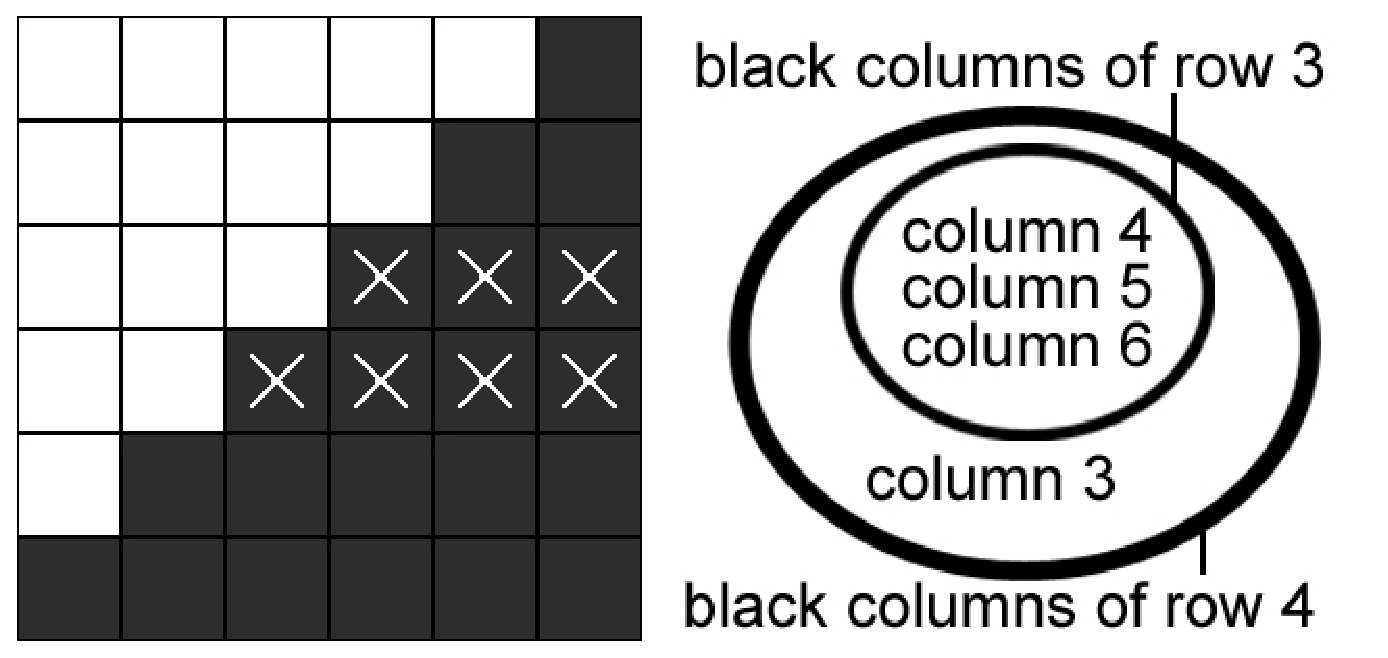
\includegraphics[height=4cm]{monotonicity_example_good}
\caption{A pattern that follows the Monotonicity Property}
\end{figure}

\begin{figure}[h]
\centering
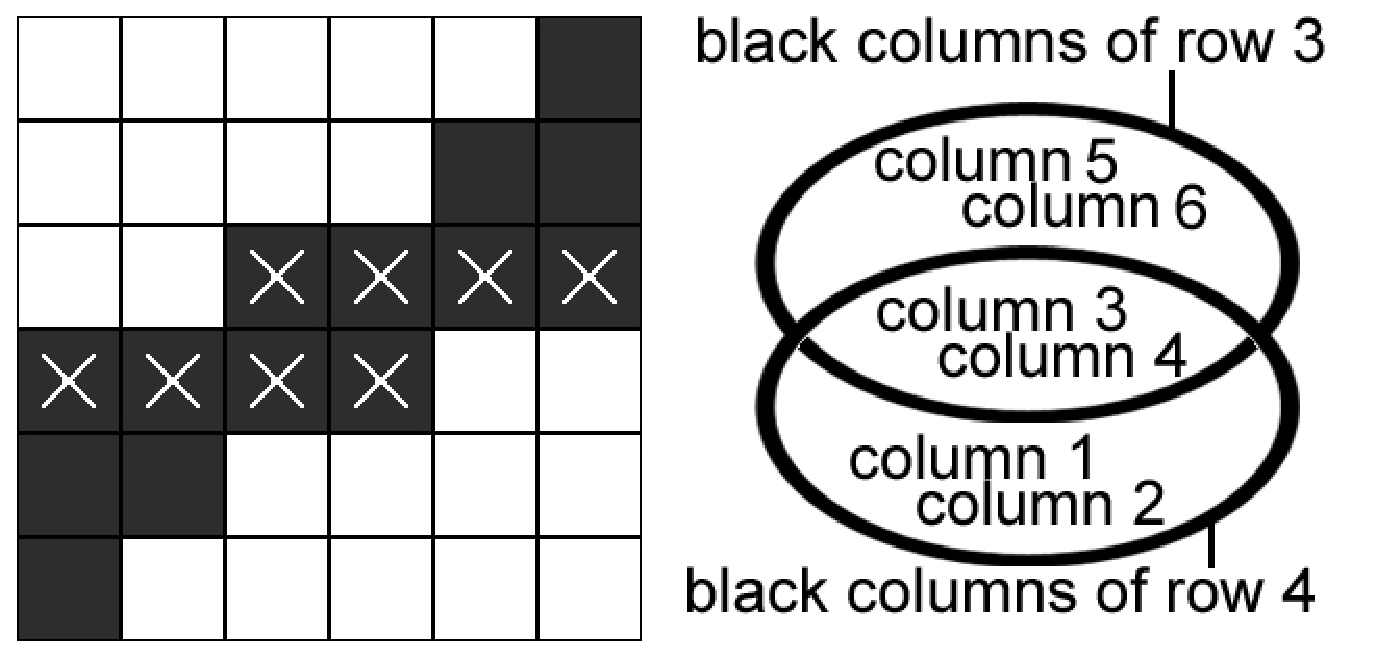
\includegraphics[height=4cm]{monotonicity_example_bad}
\caption{A pattern that does not follow the Monotonicity Property}
\end{figure}

\end{theorem}

This theorem will allow us to order the columns and rows of a strip-rule pattern P in a non-decreasing sequence regarding the number of black cells. Once the $i$-th black cell is achieved in the sequence, that $i$-th cell will remain black until the end of the sequence.


Since Theorem 3.1 of \cite{ACJKLW07} is not proven in their conference version,
we include a proof for the sake of completeness.
\begin{proof}

Let's begin our proof by verifying that items (i) and (ii) of the Monotonicity Property are equivalent.


I.) $(i) \leftrightarrow (ii)$

Let's start by proving that $\neg (i) \rightarrow \neg (ii)$. Suppose (i) does not hold. Then, given $c \in \{black, white\}$, there are two rows A and B , $A \neq B$, of $P$ that do no follow the property mentioned above. Without loss of generality, let's say $c = black$. Since one set is not contained into each other, it must be the case where both sets contains a element that the other set does not have.

This implies that both of the following are true at the same time:

\begin{enumerate}%[(a)]
\item There is a column that has a black cell on row A and a white cell on row B.
\item There is a column that has a black cell on row B and a white cell on row A.
\end{enumerate}

For reference, let's call this case a checkerboard case.

\begin{figure}[h]
\centering
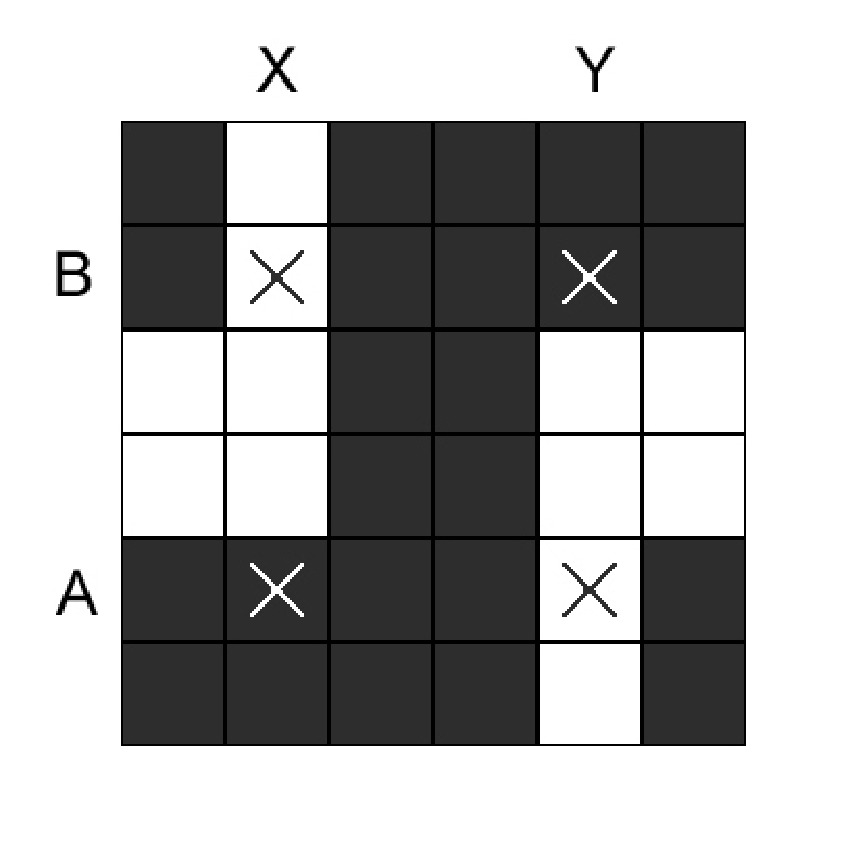
\includegraphics[height=4cm]{checkerboard_example}
\caption{Example of a checkerboard case, where (i) does not hold.}
\end{figure}

Let X and Y be one of those columns described in (a) and (b) respectively. The set of rows where black is present in X has A as one of its rows and the set of rows where black is present in Y has B as one of its rows. Hence, those sets are not contained into each other. As a result, (ii) does not hold. Thus it must be true that (ii) implies (i). ($(ii) \rightarrow (i)$)

The same argument can be made with the roles of rows and columns switched, leading to a conclusion that (i) implies (ii). ($(i) \rightarrow (ii)$) Then it must be true that (i) and (ii) are equivalent.


Let's continue with the equivalence of $P$ being a strip-rule pattern and the Monotonicity property. Let's divide the proof into two steps:

\begin{itemize}

\item ($P$ is a strip-rule pattern) $\rightarrow$ (Monotonicity Property)

We will prove that $\neg$(Monotonicity Property) $\rightarrow$ $\neg$($P$ is a strip-rule pattern). Suppose the Monotonicity property does not hold true. By contradiction, suppose that $P$ is a strip-rule pattern and let $S$ be a strip-rule RRL of size $n$ that generates $P$ such that $S = (s_{1},s_{2},\cdots,s_{n})$. 

Since the Monotonicity property does not hold true, the same argument as before for the checkerboard case can be made. Let $s_{i}$ be the last rule of $S$ that includes one of the rows or columns of the checkerboard case. Since $s_{i}$ is the last rule that they appear, no other rule after $s_{i}$ could have changed the intersection of the rows ${A,B}$ and columns ${X,Y}$ of the checkerboard case. Then, because of $s_{i}$, either A, B, X or Y must have same color cells in the checkerboard. However, if that happens, the checkerboard case does not hold anymore - a contradiction. Hence, $P$ is not a strip-rule pattern and ($P$ is a strip-rule pattern) $\rightarrow$ (Monotonicity Property) must hold true.

\item (Monotonicity Property) $\rightarrow$ ($P$ is a strip-rule pattern)


Suppose that the Monotonicity property holds. By contradiction, suppose that $P$ is not a strip-rule pattern. 
By \ref{theorem_pick_up_sticks}, the MPUS algorithm will not stop with a all-gray grid. Then it must have been stuck at a grid with no pseudo-monochromatic row or column. 

Let A be the row with the largest number of cells colored black. Since this row is not monochromatic, there must be a column Y which intersection with A is a white cell. Y must also not be pseudo-monochromatic. So there must a row B that intersects Y with a black cell. Since B has a black cell in a column that A does not have, than it must be true that the black columns of A are a subset of the black columns of B because of the Monotonicity property. Note also that those sets must not be equal. 

Hence, the number of black cells in B is higher than A, a contradiction. As a conclusion, (Monotonicity Property) $\rightarrow$ ($P$ is a strip-rule pattern) must hold, which concludes our proof.
\end{itemize}

In conclusion,  have shown that patterns generated by RRLs and patterns
that are satisfy monotonicity are equivalent.
This allows us to label the row and column classes by the number of black
cells they contain.
For example, every row that has exactly 4 black cells will be identical and
can be grouped into the class named $R_4$.
Our algorithm uses this principle to organize and determine the order of
classes to be removed.
The fact that RRL patterns have all the properties of monotonicity will
helpful is number of following proofs.
\qed
\end{proof}


% Interlacing, with proof (equiv class ordering). Also argue that
% $|Nr - Nc| \leq 1$

% Picking order lemma; leads Range search 

\subsection{Proofs Regarding Equivalence Classes}
\label{ss_classes}

This section contains some of the proofs relevant 
to the equivalence classes ordering and the creation of the 
hierarchical array of a pattern.
We point out which of these appear in \cite{ACJKLW07}, and include proofs
for completeness' sake, since \cite{ACJKLW07} omits these proofs.

\subsubsection{Active Classes}


\begin{proposition}[\cite{ACJKLW07}, Observation 6. on page 1070]
\label{t_active_classes}
During the execution of the MPUS algorithm on a black and white strip-rule pattern, there are always exactly two active classes at any given time.
The two active classes are either a row and a column
class of the same color or both classes of the same kind (rows or columns),
 being one of each color. 
\end{proposition}
%-------------------------------
Since Observation 6 of \cite{ACJKLW07} is not proven in their conference
version, we include a proof for the sake of completeness.

\begin{proof}
First, we argue that at least two classes are active. 
We use the knowledge that the Pick-Up-Sticks (PUS) algorithm will always
terminate on a gray board if an RRL solution exists.
Suppose at any time during PUS, there is only one class active.
Without loss of generality, assume this active class is a set of black rows.
We will consider the impact of picking up a black row on other potential
classes becoming active.
Picking up a black row has no impact on whether a white row becomes active.
It has no impact on a black column becoming available -- this class needs
white rows to be removed.
Finally, only once all of the black rows have been removed can a white
column class become active.
This means that picking up some or all of the active class can only result
in there either being zero active classes or still only one being active.
Contrast this with the final state of the PUS algorithm, a solid board which
translates to two active classes (a row and column of that color).
Therefore, a board with only one active class can never get to the state
with two active classes required to terminate PUS and be solvable by RRL.

Next, we argue that the 
two active classes are either a row and a column
class of the same color or both classes of the same kind (rows or columns),
 being one of each color. 
Indeed, let us first look at the case when the two  active classes are
both column classes (with a symmetric case with two row classes),
and let there be two columns $D_1$ and $D_2$ one each from these two
active classes, such that $D_1$ and $D_2$ have not been picked up.
There is a row where $D_1$ has a black cell and $D_2$
has a white cell; these cells cannot be gray
since neither $D_1$ nor $D_2$ have been picked up, and the row
has never been pseudo-monochromatic. This means $D_1$ can only
be pseudo-monochromatic as a black-gray column, and $D_2$ can only
be pseudo-monochromatic as a white-gray column.
Second, let us look at the case where the two  active classes are
one a row class and a column class, and let $D_1$ be a row from
the first active class and let $D_2$ be a column from
the second active class, such that $D_1$ and $D_2$ have not been picked up.
Then the cell at the intersection of $D_1$ and $D_2$
is not gray, and so both $D_1$ and $D_2$ are pseudo-monochromatic
with the color of this cell.

Note that the fact proved in the previous paragraph
implies that there cannot be three or more active classes:
there are not enough colors for three active column classes,
while two active columns classes and an active two class will
lead to a contradiction since both columns classes
are of the same color as the row class, while being at the same time of
different colors. Thus exactly two classes are active at any given time.
\qed
\end{proof}

%-------------------------------

\begin{proposition} [Implicit in \cite{ACJKLW07}]
\label{theorem_pick_up_altertation}
For a pattern $P$ of two colors, if one picks up all columns
of an active class, a row class of the opposite color becomes active. 
If one picks up all rows
of an active class, a column class of the opposite color becomes active. 
\end{proposition}

%-------------------------------

\begin{proof}
Since $P$ is a pattern composed of only two colors, we have that there are always two active classes at a time. Picking up a (monochromatic) column active class will not change the monochromatic property of any other column class. Hence, the class that will become monochromatic needs to be a row class. The same thing holds with the roles of rows and columns switched.

Also, the new active class must be of the opposite color because if it was not, the class becoming active would need to be already active before, since the color being removed is the same as the other cells of that class, which means that it would need to be monochromatic already.
\qed
\end{proof}

%-------------------------------

\subsubsection{Number of Equivalence Classes}

\begin{proposition} [Implicit in \cite{ACJKLW07}]
\label{theorem_difference_is_class}
Let $i$ be such that $1 \leq i < N_{C}$ and $j$ be such that $1 \leq j < N_{R}$.
\begin{enumerate}[a)]
\item Let $S_i$ be the set of rows that have white cells on the intersections of the columns of $C_{x_{i}}$ and black cells on intersection of the columns of $C_{x_{i+1}}$. $S$ is a row class ($S_i \in R$).
\item Let $S_j$ be the set of columns that have white cells on the intersections of the rows of $R_{y_{j}}$ and black cells on intersection of the columns of $R_{y_{j+1}}$. $S_j$ is a column class ($S_j \in C$).
\end{enumerate}
\end{proposition}

%-------------------------------

\begin{proof}[Proof of item (a)]
Let $i$ be such that $1 \leq i < N_{C}$ and $S$ be as the set described in 
the statement of the proposition.
Let $\alpha$, $\beta$ $\in S$.
By contradiction, suppose $\alpha$ and $\beta$ differ from each other. Let $\gamma$ be one of the columns that they differ and $k \in \mathbb{N}^{*}$ be such that $C_{x_{k}}$ is the class of $\gamma$.
Without loss of generality, assume $C_{x_{k}}$ has a black cell on the row $\alpha$ and a white cell on the row $\beta$.

Because of monotonicity, the fact that $C_{x_{k}}$ has a black cell on $\alpha$ and $C_{x_{i}}$ has a white cell on $\alpha$ implies that $x_{k} > x_{i}$ must hold true. At the same time, the fact that $C_{x_{k}}$ has a white cell on $\beta$ and $C_{x_{i+1}}$ has a black cell on $\beta$ implies that $x_{k} < x_{i+1}$ must hold true. Hence, $x_{i} < x_{k} < x_{i+1}$.

However, $x_{i} < x_{k} < x_{i+1}$ implies that $i < k < i+1$, which is a contradiction because $k \in \mathbb{N}^{*}$. $\bot$

Hence, $\alpha$ and $\beta$ do not differ from each other, which implies that $S_{i}$ is a row class ($S_{i} \in R$).

The proof of item $(b)$ follows analogously with the roles of rows and columns switched.
\qed
\end{proof}

%-------------------------------

\begin{proposition}
\label{lemma_num_rows_col_differ_one}
The number of row classes and the number of column classes differ by one. That is $\lvert N_{R} - N_{C} \rvert \leq 1$.
\end{proposition}

%-------------------------------

\begin{proof}
Let $A = max(N_{R},N_{C})$ and $B = min(N_{R},N_{C})$. 
Note that $\lvert N_{R} - N_{C} \rvert = A - B$. 
If $N_{R} = N_{C}$, we have that 
$\lvert N_{R} - N_{C}  \rvert = \lvert 0 \rvert = 0 \leq 1$.

Now, suppose $N_{R} \neq N_{C}$. Assume $A = N_{C}$. It follows that $B = N_{R}$. 

Let $i_{1}$ be such that $1 \leq i_{1} < N_{C}$. Let $S_{i_{1}}$ be the set of rows that have white cells on the intersections of the columns of $C_{x_{i_{1}}}$ and black cells on intersection of the columns of $C_{x_{i_{1}+1}}$. According to~\autoref{theorem_difference_is_class} we have that $S_{i_{1}}$ is a row class.

Let $i_{2}$ be such that $1 \leq i_{2} < N_{C}$ and $i_{2} \neq i_{1}$. Let $S_{i_{2}}$ be the set of rows that have white cells on the intersections of the columns of $C_{x_{i_{2}}}$ and black cells on intersection of the columns of $C_{x_{i_{2}+1}}$. According to~\autoref{theorem_difference_is_class}(a) we have that $S_{i_{2}}$ is a row class.

If $i_{2} < i_{1}$, we have that $x_{i_{2}+1} \leq x_{i_{1}}$, which means that the rows of $S_{i_{2}}$ must have a black cell on its intersections with $C_{x_{i_{1}}}$ due to monotonicity. This implies that $S_{i_{2}} \neq S_{i_{1}}$ because they differ on $C_{x_{i_{1}}}$.

If $i_{2} > i_{1}$, we have that $x_{i_{2}} \geq x_{i_{1}+1}$, which means that the rows of $S_{i_{2}}$ must have a white cell on its intersections with $C_{x_{i_{1}+1}}$ due to monotonicity. This implies that $S_{i_{2}} \neq S_{i_{1}}$ because they differ on $C_{x_{i_{1}+1}}$.

Thus, for every $i$ such that $1 \leq i < N_{C}$ we have a different $S_{i}$ that is a row class. From that, we have that $N_{R} \geq N_{C} - 1 $, being $N_{C} - 1$ the number of different possibilities for $i$. Hence, $N_{C} - N_{R} = A - B \leq 1$.

Now assume $A = N_{R}$. It follows that $B = N_{C}$. Using the same reasoning with~\autoref{theorem_difference_is_class}(b), we have that $N_{R} \geq N_{C} - 1$. Hence, $N_{R} - N_{C} = A - B \leq 1$.

Therefore, it is true for any case that $ \lvert N_{R} - N_{C} \rvert \leq 1$.
\qed
\end{proof}

%-------------------------------


\subsubsection{Ordering}

\begin{proposition}
\label{corollary_hierarchical_sequence}
There is an array $E_{1}$, $E_{2}$, $\cdots$, $E_{N}$ of equivalence classes that respect the following property: given $a$ and $b$ such that $1 \leq a < b \leq N$, if $E_{a}$ and $E_{b}$ are the active classes, then for every $c$ such that $1 \leq c < a$ or $b < c \leq N$, $E_{c}$ has already been picked up. Also, if $b = a + 1$, then either $E_{a} \in R$ and $E_{b} \in C$ or $E_{a} \in C$ and $E_{b} \in R$. 
Moreover, none of the columns/rows of a class $E_c$ for $a < c < b$ are
pseudo-monochromatic.  This array is the hierarchical array of a pattern.
\end{proposition}

%-------------------------------

\begin{proof}
We know from~\autoref{t_active_classes} that there are always exactly 2 acti
ve classes during an execution of PUS.
We combine this idea with the concept of monotonicity in order to create an 
organization on the possible orders the classes are picked up in.
For the original pattern, let $A$ and $B$ be the two original active classes
.
If $A,B \in C$, we must have that one is white and the other is black.
Assume without loss of generality that $A$ is white and $B$ is black.
Then we have that $A = C_{x_{1}} = C_{0}$ and $B = C_{x_{N_{C}}} = C_{n_{R}}
$.
To build the array, we will assign $E_{1} = A = C_{x_{1}}$ and $E_{N} = B = 
C_{x_{N_{C}}}$ since A and B need to be on both ends of the array because bo
th may be active even if no other classes have been picked.
If we pick up $C_{x_{1}}$, a row class will need to become active.
Also, this class will need to be the row class with the largest number of bl
ack cells due to monotonicity.
Hence, we should assign $E_{2} = R_{y_{N_{R}}}$.
Following the same reasoning, the next member will need to be the column cla
ss with the lowest number of black cells after $C_{x_{1}}$.
Hence, we should assign $E_{3} = C_{x_{2}}$.
Analogously, if we pick up $C_{x_{N_{C}}}$, the row class with the least amo
unt of black cells will become available, this being $R_{y_{1}}$.
Hence, we should assign $E_{N-1} = R_{y_{1}}$, $E_{N-2} = C_{x_{N_{C}-1}}$ a
nd so on.

Therefore we can build this array assigning $E_{2i - 1} = C_{x_{i}}$ and $E_
{2j} = R_{y_{N_{R}-j+1}}$ for every $1 \leq i \leq N_{C}$ and $1 \leq j \leq
 N_{R}$ with $E_{N} = C_{x_{N_{C}}}$.
Given $a$ and $b$ such that $1 \leq a < b \leq N$, we have that if $E_{a}$ a
nd $E_{b}$ are the active classes, every class that comes before $E_{a}$ or 
after $E_{b}$ must have already been picked up.
Also, note that two consecutive elements of the array are not of the same ty
pe of equivalence classes (row/column).
Note also that that $E_{2N_{C} - 1} = C_{x_{N_{C}}} = E_{N}$, which means th
at $N = N_{R} + N_{C} = 2N_{C} - 1$ and $N_{R} + 1 =  N_{C}$, which agrees w
ith~\autoref{lemma_num_rows_col_differ_one}.
If $A,B \in R$ we may build this array analogously assigning $E_{2j - 1} = R
_{y_{j}}$ and $E_{2i} = C_{x_{N_{C}-i+1}}$ for every $1 \leq i \leq N_{C}$ a
nd $1 \leq j \leq N_{R}$ and $E_{N} = R_{y_{N_{R}}}$. For this case, $N_{C} 
+ 1 =  N_{R}$.

For $A$ and $B$ being of different types, let's assume the color of the activ
e classes, which is the same, is white.
We can build this array assigning $E_{2i - 1} = C_{x_{i}}$ and $E_{2j} = R_{
y_{N_{R}-j+1}}$ for every $1 \leq i \leq N_{C}$ and $1 \leq j \leq N_{R}$ wi
th $E_{N} = R_{y_{1}}$.
For this case, $E_{2N_{R}} = R_{y_{1}} = E_{N}$ and $N = N_{R} + N_{C} = 2N_
{R}$ and $N_{R} = N_{C}$, which agrees with~\autoref{lemma_num_rows_col_diff
er_one}.
If the color is black, we can build this array assigning $E_{2j - 1} = R_{y_
{j}}$ and $E_{2i} = C_{x_{N_{C}-i+1}}$ for every $1 \leq i \leq N_{C}$ and $
1 \leq j \leq N_{R}$ with $E_{N} = C_{x_{N_{C}}}$.
For this case, $E_{2N_{C}} = C_{x_{N_{C}}} = E_{N}$ and $N = N_{R} + N_{C} =
 2N_{C}$ and $N_{R} = N_{C}$.
By construction it is easy to see that a column/row of a class $E_c$ must no
t be monochromatic while the two active classes are $E_a$ and $E_b$ for $a <
 c < b$.
From our construction and definitions, the only way for a class to become ac
tive, is to have either the class immediately to its left or right in the hi
erarchical array already removed.
This therefore cannot be true while $a < c < b$ since we know the only class
es removed are those that come before $a$ or come after $b$.
\qed
\end{proof}
%-------------------------------


% Containment lemma, with citations

\subsection{Segments Properties}
\label{ss_seg}

This section contains the proofs of the properties discussed earlier regarding segments.

\subsubsection{Segment Redefinition}

Earlier, we mentioned that the definition given by "Applegate et al."'s paper
\cite{ACJKLW07} is redundant. They define a segment as being a tuple of five elements $(E_{x},c_{x},E_{y},c_{y},U)$, where $E_{x}$ and $E_{y}$ are the active equivalence classes, $c_{x}$ and $c_{y}$ are the colors of the members $E_{x}$ and $E_{y}$ (that are pseudo-monochromatic), and $U$ is the subset of members left unpicked of $E_{y}$ ($U \subset E_{y}$). The next statement shows that the colors are redundant, allowing us to reduce the definition of a segment to $(E_{x},E_{y},,U)$.

\begin{proposition}
\label{corollary_known_colors}
Let $E_{1}$, $E_{2}$, $\cdots$, $E_{N}$ be the hierarchical array of a pattern. Given $a$ and $b$ such that $1 \leq a < b \leq N$ it is possible to know what colors correspond to each active class of a label ($E_{a}$,$E_{b}$).
\end{proposition}

\begin{proof}
Given $a$ and $b$ such that $1 \leq a < b \leq N$.

\begin{itemize}
\item If $E_{1} \in C$ and $E_{N} \in C$, we have that: If $E_{a} \in C$, $E_{a}$ is white. If $E_{a} \in R$, $E_{a}$ is black. If $E_{b} \in C$, $E_{b}$ is black. If $E_{b} \in R$, $E_{a}$ is white.

\item If $E_{1} \in R$ and $E_{N} \in R$, we have that: If $E_{a} \in C$, $E_{a}$ is black. If $E_{a} \in R$, $E_{a}$ is white. If $E_{b} \in C$, $E_{b}$ is white. If $E_{b} \in R$, $E_{a}$ is black.

\item If $E_{1}$ and $E_{N}$ are from different types and $E_{1}$ and $E_{N}$ are initially black, we have that: If $E_{a} \in C$, $E_{a}$ is black. If $E_{a} \in R$, $E_{a}$ is white. If $E_{b} \in C$, $E_{b}$ is white. If $E_{b} \in R$, $E_{a}$ is black.

\item If $E_{1}$ and $E_{N}$ are from different types and $E_{1}$ and $E_{N}$ are initially white, we have that: If $E_{a} \in C$, $E_{a}$ is white. If $E_{a} \in R$, $E_{a}$ is black. If $E_{b} \in C$, $E_{b}$ is black. If $E_{b} \in R$, $E_{a}$ is white.
\end{itemize}

This happens because when we pick from either sides, the color alternates for each item picked up as well as its type. Hence, the color of $E_{a}$ will always match the color of $E_{1}$ if they have the same type and differ if they are from different types.
The same will happen with $E_{b}$ and $E_{N}$.
\qed
\end{proof}

It is a consequence of this corollary the fact that having a segment $S=(E_{k_{1}},c_{k_{1}},E_{k_{2}},c_{k_{2}},U)$, $U \subset E_{k_{2}}$, is redundant. We may start referring to a segment as only $S=(E_{k_{1}},E_{k_{2}},U)$, $U \subset E_{k_{2}}$.

\subsubsection{}
\begin{proposition} [statement 2(a) of Lemma 4.2 of \cite{ACJKLW07}]
\label{p_embed}
%Suppose we have two sets $U_x$ and $U_y$
%of active blocks of the two active classes $E_x$ and $E_y$.
%Assume after picking up some sticks,
%$E_z$ suplants $E_x$  as an active class, while $E_y$ remains active,
%and this is done picking up the minimum number of sticks.
%Then one optimum solution is to pick up all the blocks of $E_y$
%embedded into $E_x$, followed by picking up the resulting
%maximal sticks of $E_x$.
Suppose we have two sets $U_x$ and $U_y$
of active blocks of the two active classes $E_x$ and $E_y$.
Suppose there is an optimal solution that completely picks up $E_x$ before
completely picking up $E_y$.
Then there also exists an optimal solution that picks up all embedded
members of $E_y$ before picking up $E_x$.
\end{proposition}
Since Lemma 4.2 of \cite{ACJKLW07} is not proven in their conference version,
we include a proof for the sake of completeness.
\begin{proof}
This follows closely from the definition of embedded members, which can be
effectively picked up at zero net cost along with the blocks embedding them.
This is easy to observe in an example: consider the leftmost three columns
of Fig.~\ref{fig:embedment_example}.
Here we see a member of $C_0$ (the white column) embedded in two blocks of
$C_2$.
We could pick up the embedding blocks using two rules, or we could first
pick up the embedded block followed by picking up both embedding blocks
using only one wider rule.
The overall result is still two rules which pick up all members of the
embedding class.
This is, without loss of generallity, either a helpful or irrelevant action.
So in our solution we will always choose to remove the embedded blocks
before the embedding blocks.
\qed
\end{proof}


\subsubsection{Containment Lemma} [Lemma 4.3 of \cite{ACJKLW07}]
\label{ss_cont}
Let $S$ and $S'$ be two segments on the same equivalence classes, then either $U \subset U'$ or $U' \subset U$.

Intuitively,
this follows from the fact that we have a strict ordering on the equivalence classes that could embed columns in $U$. See "Applegate et al."'s paper
\cite{ACJKLW07} for a rigorous inductive proof of this lemma by the same name.


%ignoring segment with empy set U

%Graph does not have cycles



\end{document}
